
\input{preambulo}

\begin{document}

%%%%%%%%%%%%%%%%%%%%%%%%%
% Aquí va la portada
%%%%%%%%%%%%%%%%%%%%%%%%%

\begin{titlingpage} % Portada

    \raggedleft % Alineada a la derecha
    %\raggedright % Alineada a la izquierda
	
	\vspace*{\baselineskip} % Whitespace at the top of the page
	
	\vspace*{0.25\textheight} % Whitespace before the title
	
	%------------------------------------------------
	%	Cosas del título
	%------------------------------------------------
    
    \vspace*{0.1\textheight}

    {\Huge{\textbf{Matemáticas Financieras}}}\\[\baselineskip] % Aquí va el título
    \vspace*{0.1\textheight}

    %------------------------------------------------
	%	Aquí van los nombres
	%------------------------------------------------
    
    {\Large Eduardo Selim Matínez Mayorga}\\[\baselineskip]
	
	\vfill

\end{titlingpage}

\thispagestyle{empty}

\chapter*{Teoría del interés} % Capítulo TI

\textbf{Definición de Interés:} El interés se puede definir como una compensación/beneficio que una parte A le da a una parte B por dejar de satisfacer una necesidad para que el otro satisfaga la propia.

Solo pensando en términos monetarios... ¿Por qué las inversiones (en teoría ) crecen?

Algunos factores que intervienen en una inversión:

\begin{itemize}
\item Dinero (¿cuánto tiempo?)
\item ¿En qué se invierte?
\item ¿Cuánto tiempo lo invierto?
\item Inflación
\item Bajo que condiciones contractuales lo invierto (¿cómo crece el dinero ?)
\item Oferta y demanda
\item ¿Cuándo lo invierto?
\end{itemize}

Por un momento(grande) pensemos que el nivel de inversión depende solo del tiempo.

\begin{definition}
Se dice que una función $a:\left[ 0,\infty \right) \longrightarrow \RR_+ $ es una función de \textbf{acumulación} si cumple:

\begin{enumerate}
\item  $a(0) = 1$
\item $a\left(\cdot\right)$ es no-decreciente
\item $a(\cdot)$ es continua por la derecha y con límite por la izquierda.
\end{enumerate}
\end{definition}

$a(t)$ representa el valor acumulado de $\$1$ que hay durante un lapso de tiempo t.

\newpage

\textbf{Ejemplo:}
\begin{enumerate}
\item $a(t) = 1+ct$, $c>0$, $c$ constante (interés simple)
\item $a(t) = e^{\alpha t}$, $\alpha > 0$ (interés compuesto)
\item $a(t) = ct^2 + 1$, $c>0$
\item $a(t) = 1$
\item $a(t) = (1+t)^c$, $c>0$
\item $a(t) = 1 + arctang(t)$
\item $a(t) = \sqrt{t+1}$
\item $a(t) = \sqrt{t} + 1$
\item $a(t) = 1 + c\left[ t \right]$
\item $a(t) = e^{\left[ t \right]}$
\end{enumerate}

\begin{definition}
Se define la \emph{\textbf{función de monto}} correspondiente a $a(t)$ como un capital inicial $k>0$, como 
$$ A_k \left( t \right) : = k \cdot a \left( t\right)  $$
\end{definition}

\begin{remark}
Se cumple (1) y (3), pero $A_k(0) = k \cdot a(0) = k \cdot 1 = k$
\end{remark}

$A_k(t)$ representa el valor acumulado de una inversión de un lapso de tiempo t.

\textbf{Representación gráfica:}

\begin{center}
    \begin{tikzpicture}
        % draw horizontal line   
        \draw (-5,0) -- (4,0);
    
    
    % draw vertical lines
    \foreach \x in {-5,4}
    \draw (\x cm,3pt) -- (\x cm,-3pt);
    
    % draw nodes
    \draw (-5,0) node[below=3pt](a) {$ 0 $}
    node[below =3pt of a]{\textdollar $1$}
     node[above=3pt] {$  $};
     \draw (4,0)node[below=3pt](a) {$ t $}
	  node[below=3pt of a]{tiempo}
	  node[above=3pt] {$ a(t) $};
	  
\path [draw=black,postaction={on each segment={end arrow=black}}]
  (-5,0) to [bend left] (3.6,0.5);
\end{tikzpicture}
\end{center} 

\begin{center}
    \begin{tikzpicture}
        % draw horizontal line   
        \draw (-5,0) -- (4,0);
    
    
    % draw vertical lines
    \foreach \x in {-5,4}
    \draw (\x cm,3pt) -- (\x cm,-3pt);
    
    % draw nodes
    \draw (-5,0) node[below=3pt](a) {$ 0 $}
    node[below =3pt of a]{\textdollar $k$}
     node[above=3pt] {$  $};
     \draw (4,0) node[below=3pt](a) {$ t $}
	  node[below=3pt of a]{tiempo}     
      node[above=3pt] {$ A_k(t) $};
      
\path [draw=black,postaction={on each segment={end arrow=black}}]
  (-5,0) to [bend left] (3.6,0.5);         
\end{tikzpicture}
\end{center} 
     
¿Cómo medimos el performance de una función de acumulación o función de monto?

Estudiaremos 3 indicadores:
\begin{enumerate}
\item Tasa efectiva de interés al tiempo t
\item Tasa de descuento al tiempo t
\item Fuerza de interés
\end{enumerate}

\begin{definition}
Para una función de acumulación $a\left( \cdot \right)$ se define la tasa efectiva de \underline{\textbf{interés al tiempo t}} como:
$$ i_t := \frac{a\left( t \right) - a\left( t -1 \right)}{a\left( t - 1 \right)}$$
\end{definition}

\textbf{Interpretación:} Por cada peso invertida al tiempo $t-1$ hay $i_t$ unidades de ganancia. "Lo que yo gané por cada peso que invertí".

\textbf{Ejemplo:}
\begin{enumerate}
\item Para $a(t) = 1 + ct$

$i_t = \frac{a\left( t \right) - a\left( t -1 \right)}{a\left( t - 1 \right)} = \frac{1 + ct - \left[ 1 + c(t-1)\right] }{1+c(t-1)} = \frac{c}{1+c(t-1)}$

Obsérvese que la aplicación $t \longmapsto i_t = \frac{c}{1+c(t-1)}$ es \underline{decreciente}.

Con la función $a(t) = 1 + ct$ ganamos, pero cada vez menos conforme el tiempo avanza.
\item Para $a(t) = e^{\alpha t}$, $\alpha > 0$

$i_t = \frac{a\left( t \right) - a\left( t -1 \right)}{a\left( t - 1 \right)} = \frac{e^{\alpha t} - e^{\alpha (t-1)}}{e^{\alpha (t-1)}} = \frac{e^{\alpha (t-1)}\left[ e^{\alpha}-1\right]}{e^{\alpha (t-1)}} = e^{\alpha} -1$

Obsérvese que la aplicación $t \longmapsto i_t = e^{\alpha} -1$ es \underline{constante}.

\textcolor{red}{Tarea}

Para $a(t)= e^{t^2}$ calcular $i_t$ y ver si $t \longmapsto i_t$ es creciente o decreciente

\item $a(t) = (1+c)^t$, $c > 0$

$i_t =  \frac{a\left( t \right) - a\left( t -1 \right)}{a\left( t - 1 \right)} = \frac{(1+c)^t - (1+c)^{t-1}}{(1+c)^{t-1}} = \frac{(1+c)^{t-1}[(1+c)-1]}{(1+c)^{t-1}} = 1+c-1 = c $

Obsérvese que la aplicación $t \longmapsto i_t = e^{\alpha} -1$ es \underline{constante}.
\end{enumerate}

\begin{remark}
Los ejemplos 2. y 3. son el mismo.

$(1+c)^t=e^{log\left((1+c)^t \right)} = e^{tlog(1+c)}=e^{\alpha t}$, con $\alpha = log(1+c)$.

En el mundo financiero preferimos escribir a la función exponencial como $(1+c)^t$.
\end{remark}

\underline{\textcolor{blue}{Notación}}

En realidad preferimos escribir a la función exponencial como $a(t) = (1+i)^t$. Bajo esta notación $i_t = c = i$, es decir, $i_t=i$.

Al número "$i$"  le llamamos \textcolor{blue}{tasa efectiva de interés}, y al modelo $a(t)=(1+i)^t$ se le conoce como el \underline{\textcolor{blue}{modelo de interés compuesto}}.

\begin{remark}
$\frac{A_k(t)-A_k(t-1)}{A_k(t-1)}=\frac{ka(t) - ka(t-1)}{ka(t-1)} = \frac{a(t)-a(t-1)}{a(t-1)} = i_t$
\end{remark}

\begin{definition}
Para una función de acumulación $a(t)$ diferenciable, se define la \underline{\textcolor{blue}{fuerza de interés}} correspondiente a $a(\cdot)$ como 
\begin{equation*}
\boxed{
\delta_t : = \frac{\frac{\partial}{\partial t} a(t)}{a(t)}
}
\end{equation*}

¿De dónde viene esa definición?
% Se puede mejorar la h que tiende a 0 
$$\frac{\frac{\partial}
{\partial t} a(t)}{a(t)} \mathrel{\stackon[1pt]{$\approx$}{$h \approx 0$}} \frac{\frac{a(t+h)-a(t)}{h}}{a(t)} = \frac{a(t+h)- a(t)}{ha(t)}$$


\end{definition}

\begin{remark}
$\delta_t$ también se puede obtener como $\frac{\partial}{\partial t} log(a(t)) = \frac{a'(t)}{a(t)} = \delta_t$
\end{remark}

\textbf{Ejemplo: }
\begin{enumerate}
\item $a(t)=e^{\alpha t}$

$\delta_t = \frac{a'(t)}{a(t)} = \frac{\left( e^{\alpha t}\right)'}{e^{\alpha t}} = \frac{\alpha e^{\alpha t}}{e^{\alpha t}} = \alpha$         

$\therefore \delta_t = \alpha$, con $\alpha$ constante
\item $a(t) = 1+ct$

$\delta_t = \frac{a'(t)}{a(t)} = \frac{\left( 1+ct\right)'}{1+ct} = \frac{c}{1+ct}$ 

$\therefore t\longmapsto \delta_t$ es decreciente
\end{enumerate}

\begin{definition}
Para una función de acumulación $a(\cdot )$ se define la \textcolor{blue}{\underline{tasa efectiva de descuento al tiempo t}} como:
\begin{equation*}
\boxed{d_t := \frac{a(t)-a(t-1)}{a(t)}}
\end{equation*} 
\end{definition}

También se conoce como tasa efectiva de descuento en el intervalo $\left[ t-1, t\right] $. ¿Cómo se interpreta $d_t$?

Por cada unidad de $a(t)$ hay $d_t$ unidades de $a(t)-a(t-1)$. "Por cada peso obtenido hay $d_t$ pesos de ganancia obtenida".

\textbf{Ejemplo:}
\begin{enumerate}
\item $a(t) = (1+i)^t$

$d_t = \frac{a(t) - a(t-1)}{a(t)} = \frac{(1+i)^t - (1+i)^{t-1}}{(1+i)^t} = 1 - (1+i)^{-1} = \frac{1+i-1}{1+i} = \frac{i}{1+i} = c$

donde $c$ es una constante
\item $a(t) = 1+it$

$d_t = \frac{a(t) - a(t-1)}{a(t)} = \frac{1 + it - (1 + i(t - 1))}{i + it} = \frac{i}{1 + it}$
\end{enumerate}

\begin{remark}
La aplicación $t \longmapsto d_t = \frac{i}{1 + it}$ es \underline{decreciente}.
\end{remark}

\begin{enumerate}
\item[1)] Supongamos que un banco le ofrece darte un porcentaje $c$ por cada cada peso invertido al final de cada periodo, \underline{sin} posibilidad de reinvertir las ganancias.

¿Cuánto dinero tendré al final de $n$ periodos? Supongamos que hoy invertimos $K$.
\begin{itemize}
\item[$\longrightarrow$] ¿Cuánto dinero tendré al final de 1 periodo?
\[  \underbrace{K}_{\text{Inicial}} + \underbrace{Kc}_{\text{Ganancia}} = K(1+c)\]
\item[$\longrightarrow$] ¿Cuánto dinero tendrá al final de 2 periodos?
\[ \underbrace{K(1+c)}_{\text{Ya lo tenía}} + \underbrace{Kc}_{\text{Ganancia}} = K(1+2c)\]
\end{itemize}
Inductivamente, el dinero al final de $n$ periodos es $K(1+n\cdot c)$, $n\in \NN_+$.
\item[2)] Ahora, con la posibilidad de reinvertir las ganancias:

Supóngase que un banco le ofrece darle un porcentaje por cada peso invertido al final de cada periodo \underline{con} posibilidad de reinvertir las ganancias.
\begin{itemize}
\item[$\longrightarrow$] ¿Cuánto dinero tendré al final de 2 periodos?
\[ \underbrace{K(1+c)}_{\text{Ya lo tenía}} + \underbrace{K(1+c)\cdot c}_{\text{Ganancia}} = K(1+c)(1+c) = K(1+c)^2\]
\item[$\longrightarrow$] ¿Cuánto dinero tendré al final de 3 periodos?
\[ \underbrace{K(1+c)^2}_{\text{Ya lo tenía}} + \underbrace{[K(1+c)^2]c}_{\text{Ganancia}} = K(1+c)^2(1+c) = K(1+c)^3\]

Inductivamente el dinero al final de $n$ periodos es $k(1+c)^n$, $n\in \NN_+$.
\bigskip
\item[$\longrightarrow$] A 1) se le conoce como la \textcolor{blue}{\underline{génesis económica del interés simple}}, $a(n) = 1+cn$, y nos gusta escribirla como $a(n) = 1+in$, donde a $i$ se le llama \textcolor{blue}{tasa efectiva de interés simple}.
\item[$\longrightarrow$] A 2) se le conoce como \textcolor{blue}{\underline{génesis económica del interés compuesto}}, $a(n) = (1+c)^n$, y nos gusta escribirla como $a(n) = (1+i)^n$, donde a $i$ se le conoce como \textcolor{blue}{tasa efectiva de interés}.
\end{itemize}
\end{enumerate}
\newpage
\begin{definition}
Se dice que una función de acumulación $a(\cdot )$ es un \textcolor{blue}{\underline{modelo de interés simple}} si cumple las siguientes características:
\begin{enumerate}
\item[(1)] $a(1) = 1+ i$, para $i$ constante
\item[(2)] $a(\cdot)$ es diferenciable
\item[(3)] $\forall s,t \in \left[0,\infty \right) \quad a(t+s)+1 = a(t) + a(s) \ldots (\Laughey)$
\end{enumerate}
\end{definition}

\begin{proposition}
Si $a(\cdot)$ es una función de acumulación que es un modelo de interés simple, entonces $a(t) = 1 + it \quad \forall t\in \left[0,\infty \right)$
\end{proposition} 

\begin{proof}
\begin{align*}
a'(u) &= \lim\limits_{h \to 0} \frac{a(u+h)-a(u)}{h} \longleftarrow \, \text{Existe por (2)} \\
&\stackrel{\mathclap{\normalfont\mbox{(\Laughey)}}}{=} \lim\limits_{h \to 0} \frac{\left(a(u)+a(h)-1 \right) - a(u)}{h}\\
&= \lim\limits_{h \to 0} \frac{a(h)-1}{h}\\
&= \lim\limits_{h \to 0} \frac{a(h)-a(0)}{h}\, \text{, pues} \, a(\cdot) \, \text{es función de acumulación}\\
&= a'(0) = \text{cte} \, \text{con respecto a t.}
\end{align*}

Es decir, $a'(u) = a'(0)\Longrightarrow \int_{0}^{t}a'(u)\,du = \int_{0}^{t}a'(0)\,du$
\begin{align*}
&\stackrel{\mathclap{\normalfont\mbox{\text{TFC}}}}{\Longrightarrow} a(t) - a(0) = a'(0)\cdot t\\
&\Longrightarrow a(t) - 1 = a'(0)\cdot t\\
&\Longrightarrow a(t) = 1 + a'(0)t \ldots (*)\\
\text{Pero por (1)} \, &\Longrightarrow a(1) = 1+i = 1 + a'(0)\cdot 1\\
& \Longrightarrow a'(0) = i
\end{align*}
Sustituimos en $(*)$
$$\therefore \, a(t) = 1+it$$
\end{proof}

\begin{definition}
Se dice que una función de acumulación $a(\cdot)$ es un \textcolor{blue}{\underline{modelo de interés compuesto}} si cumple las siguientes características:
\begin{enumerate}
\item[(1)] $a(1) = 1+i$, para $i$ constante
\item[(2)] $a(\cdot)$ es diferenciable
\item[(3)] $\forall s,t \in \left[0,\infty \right) \quad a(t+s)= a(t)\cdot a(s) \ldots (\Neutrey)$
\end{enumerate}
\end{definition}
\newpage 
\begin{proposition}
Si $a(\cdot)$ es una función de acumulación que es un modelo de interés compuesto, entonces $a(t) = (1+i)^t \quad \forall t\in \left[0,\infty \right)$
\end{proposition}

\begin{proof}
\begin{align*}
a'(u) &= \lim\limits_{h \to 0} \frac{a(u+h)-a(u)}{h} \longleftarrow \, \text{Existe por (2)} \\
&\stackrel{\mathclap{\normalfont\mbox{(\Neutrey)}}}{=} \lim\limits_{h \to 0} \frac{a(u)\cdot a(h) - a(u)}{h}\\
&=  a(u) \cdot \lim\limits_{h \to 0} \frac{a(h)-1}{h}\\
&=  a(u) \cdot \lim\limits_{h \to 0} \frac{a(h)-a(0)}{h}\, \text{, pues} \, a(\cdot) \, \text{es función de acumulación}\\
&= a(u)\cdot a'(0)
\end{align*}
\[\therefore \, a'(u) = a(u) \cdot a'(0) \Longrightarrow \frac{a'(u)}{a(u)} = a'(0)\]

$$\Longrightarrow \int_{0}^{t}\frac{a'(u)}{a(u)}\, du = \int_{0}^{t} a'(0)\, du \Longrightarrow \int_{0}^{t} \frac{\partial}{\partial t} log(a(u)) \, du = a'(0)t$$
\begin{align*}
&\stackrel{\mathclap{\normalfont\mbox{\text{TFC}}}}{\Longrightarrow} log(a(t)) - log(a(0)) = a'(0)t\\
&\Longrightarrow log(a(t)) - \cancelto{0}{ log(1)} = a'(0)t\\
&\Longrightarrow a(t) = exp\{a'(0)t\} \ldots (\text{\ding{164}})
\end{align*}
Pero por (1), $a(1) = 1+i$

Sustituimos en (\ding{164}) 
\begin{align*}
&1+i = exp\{a'(0)\cdot 1\} \\
&\Longrightarrow log(1+i) = a'(0) \ldots (\#)\\
&\text{Sustituyendo}\,(\#)\, \text{en} \, (\text{\ding{164}})\\
& \Longrightarrow a(t) = exp\{log(1+i)\cdot t\}\\
& \Longrightarrow a(t) = exp\{log(1+i)^t\}\\
& \therefore \, a(t) = (1+i)^t
\end{align*}
\end{proof}
\newpage
\textbf{Ayudantía}

$\frac{d}{dt}(1+i)^t = \frac{d}{dt} \left(e^{t\log(1+i)} \right)= e^{t\log(1+i)}\left(\log(1+i)\right) =\underline{(1+i)^t\left( \log(1+i)\right)}$

\begin{theorem}[Teorema de Taylor]
Sea $f$ una función, supongamos que existen $f', \, \ldots \, f^{(n+1)}$ en $[a,x], \, a\in\RR$. Sea $n\in\NN$, se define como:
$$f(x) = \frac{f(a)}{0!}+\frac{f'(a)}{1!}(x-a)+\frac{f''(a)}{2!}(x-a)^2 + \, \ldots \, + \frac{f^{(n)}(a)}{n!}(x-a)^n + R_{n, a(x)}$$
Entonces $R_{n, a(x)} = \frac{f^{(n+1)}(a)}{(n+1)!}(x-a)^n$ y si $f$ es integrable
$R_{n, a(x)} = \int\frac{f^{(n+1)}(t)}{(n+1)!}(x-t)^n\, dt$.
\end{theorem} 

\hfill

\begin{multicols}{2}
\underline{Series geométricas} 
\begin{align*}
& 1 + (1+i) +(1+i)^2 + \, \ldots \, + (1+i)^n\\
& 1 + a + a^2 + \, \ldots \, a^{n-1} = S\\
& a + a^2 + a ^3 + \, \ldots \, + a^n = aS\\
& S - aS \Longrightarrow 1 + a - a + a^2 - a^2 + \, \ldots \, - a^n\\
& S - aS = 1-a^n
\Longrightarrow S = \frac{1-a^n}{1-a}
\end{align*}
Además
\begin{itemize}
\item[*] Si $a=1\, \Longrightarrow \, S_{n=1} = n$
\item[*] Si $a\neq 1\, \Longrightarrow \, S_n = \frac{1-a^n}{1-a} = \frac{a^n-1}{a-1}$

$|a|<1$ Converge $= \frac{1}{1-a}$
\end{itemize}
\columnbreak
\underline{Telescópicas}
\begin{align*}
&\sum_{n=1}^{N} \, \frac{1}{n(n-1)} = \sum_{n=1}^{N} \, \left(\frac{1}{n} -\frac{1}{n+1} \right) \\
& = \left(1-\frac{1}{2} \right) + \left(\frac{1}{2} - \frac{1}{3}\right) +\, \ldots \, + \left(\frac{1}{N} - \frac{1}{N+1}\right)\\
& = 1- \frac{1}{N+1}\\
& \text{Ahora si} \, N \longrightarrow \infty\\
& \sum_{n=1}^{N}\left(\frac{1}{n(n+1)} \right) \longrightarrow 1 
\end{align*}
\end{multicols}

\hfill

\begin{remark}
\begin{align*}
&\int v^t \, dt = 1 \cdot \int v^t \, dt = \frac{\log (v)}{\log (v)}\int v^t \, dt & u = v^t \quad du = v^t \log(v)\\
&\Longrightarrow \frac{1}{\log (v)}\int v^t\log(v) \, dt =\frac{v^t}{\log(v)} + C & \Longrightarrow \int du = \int v^t \log(u) = v^t
\end{align*}

En general: 
\begin{align*}
& \int u'\cdot e^{u}\, du = e^{u} + C \\
& \int u'a^{u} \, du = \frac{a^{u}}{\log(a)} + C 
\end{align*}
\end{remark}
\newpage
\textbf{\underline{Ejercicios} }(Interés simple)

\begin{enumerate}
\item ¿Cuánto interés se gana en el cuarto año si se invierten $\$ 3000$ bajo interés simple a una tasa anual del $5\%$ ¿Cuál es el saldo al final del cuarto año?

Saldo final:

$A(t) = 3,000(1+0.05(4)) = \underline{3,600}$

\item ¿En cuántos años se acumularán $\$500$ a $\$800$ con un interés del $6\%$?

$A(1) = 500, \: A(t) = 800, \: i = 6\% \\
A(t) = 500 (1 + 0.06(t)) = 800\\
\frac{800}{500} = 1+ 0.06 (t) \: \Longrightarrow \: \frac{8}{5}-1 = 0.06(t) \: \Longrightarrow \: \frac{\frac{8}{5}-1}{0.06} = t \quad  \therefore\underline{\: t = 10 \, \text{años}} $

\item Encuentre la tasa de interés simple anual para que $\$ 1,000$ invertido a tiempo $t = 0$ crezca a $\$1,700$ en 8 años.

$A(0) = 1,000, \: A(8) = 1,700, \: t=8 \, \text{años}\\
A(8) = 1,000(1+i(8)) = 1,700 \: \Longrightarrow \: \frac{1,700}{1,000} = (1+i(8))\\
\Longrightarrow \: \frac{(1.7-1)}{8} = i = 0.087\\
\therefore \: \underline{\text{La tasa anual debe ser de } 8.7\%}$

\item A una tasa de interés simple, $\$ 1,200$ invertidos en el tiempo $t = 0$ acumula $\$1,320$ en $t$ años. Encuentre el valor acumulado de $\$500$ invertido a la misma tasa de interés simple y a $t = 0$, pero esta vez para $2t$

$A(0) = 1,200, \: A(t) = 1,320$
\begin{enumerate}
\item $A(t) = 1200(1+it) = 1320 \: \Longrightarrow \: t = \frac{\frac{1320}{1200}-1}{i}$
\item $A(2t) = 500(1+i2t)\\
500\left( 1+\cancel{i}2\left( \frac{\frac{1320}{1200}-1}{\cancel{i}}\right) \right) = 500 \left( 1 + 2 \left( \frac{1320}{1200} -1\right) \right) = \underline{600\, \text{acum}}  $
\end{enumerate}
\end{enumerate}

\textbf{\underline{Ejercicios}} (Interés compuesto)

\begin{enumerate}
\item Alice invierte $\$2,200$, Su inversión crece de acuerdo al interés compuesto con una tasa de interés anual de $4\%$ por $t$ años en el cual acumuló $\$8,000$. Encuentre $t$.

$A(0) = 2,200,\: i=4\%,\: A(t) = \$ 8,000 \\
\hfill \\
A(t) = 2,200(1+0.04)^t = 8,000 \: \Longrightarrow \: (1+0.04)^t = \frac{8,000}{2,200} \\
\Longrightarrow \: t\ln(1+0.04) = \ln\left( \frac{8,000}{2,200}\right) \\
\Longrightarrow t = \frac{\ln\left(\frac{8,000}{2,200} \right) }{\ln(1.04)}\\
\hfill\\
\therefore \: \underline{t=32.91}$
\newpage
\item Eliot recibe la herencia de su tía Ruth, cuando ella murió en su cumpleaños número 5. En su cumpleaños 18, la herencia creció a $\$ 32,168$. Si el dinero ha estado creciendo a una tasa de interés compuesto anual de $6.2\%$ encuentre la cantidad que le heredó la tía Ruth a Eliot.

$A(0) = M,\: i = 6.2\%,\: A(13) = 32,168\\
\hfill
\\
A(0) = M(1.062)^{13} = 32,168 \: \Longrightarrow \: M\frac{32,168}{(1.062)^{13}} = \underline{14,716.52}$

\item ¿Cuánto interés se gana en el cuarto año de una inversión de $\$1,000$ invertida a una tasa compuesta anual efectiva de $5\%$ ?

$t = 4\, \text{años}, \: M=1,000,\: i = 5\% \\
\hfill \\
A(4) = 1,000(1+0.05)^4 = 1,215.5 \: \Longrightarrow \: 1,215.5 - 1,000 = 215.5\\
\therefore \: \underline{\text{El interés ganado es} \, \$ 215.5}$
\item A una cierta tasa de interés compuesta, el dinero se duplicará en $\alpha$ años, se triplicará en $\beta$ años y se multiplicará por 10 en $\gamma$ años. Al mismo tiempo con una tasa de interés compuesta, $\$5$ incrementa a $\$12$ en $n$ años. Encuentre el interés $a$, $b$, $c$ tal que $n=a\alpha + b\beta + c\gamma$
\begin{align*}
& A(\alpha) = M(1 + i)^{\alpha} = 2M  & \hfill \hfill \\
& A(\beta) = M(1+i)^{\beta} = 3M  & \textcolor{red}{\text{Tarea:}} \, A(n) = 5 (1+i)^n = 12 \\
& A(\gamma) = M(1+i)^{\gamma} = 10M
\end{align*}
\item Eduardo depositó $\$ 826$ en una cuenta de ahorros que genera intereses a una tasa de incremento del banco. Durante los primeros $3$ años del depósito la tasa de interés anual es del $2.6\%$. Para los próximos $2$ años la tasa efectiva anual es del $4.5\%$ y los siguientes $5$ años la tasa de interés efectiva anual es del $6\%$, ¿Cuál es el acumulado al final de $10$ años?

\begin{center}
    \begin{tikzpicture}
        % draw horizontal line   
        \draw[->] (-5,0) -- (6,0);
    
    
    % draw vertical lines
    \foreach \x in {-5,...,5}
    \draw (\x cm,3pt) -- (\x cm,-3pt);
    
    % draw nodes
    \draw (-5,0) node[below=3pt]{$ 0 $};
    \draw (-4,0) node[below=3pt]{$ 1 $};
    \draw (-3,0) node[below=3pt](a){$ 2 $} 	node[below = 3pt of a]{$ X $};
    \draw (-2,0) node[below=3pt]{$ 3 $};
    \draw (-1,0) node[below=3pt]{$ 4 $};
    \draw (0,0) node[below=3pt](a){$ 5 $} 	node[below = 3pt of a]{$ Y $};
    \draw (1,0) node[below=3pt]{$ 6 $};
    \draw (2,0) node[below=3pt]{$ 7 $};
    \draw (3,0) node[below=3pt]{$ 8 $};
    \draw (4,0) node[below=3pt]{$ 9 $}; 
    \draw (5,0) node[below=3pt]{$ 10 $};
    
  	\path [draw=black,postaction={on each segment={end arrow=black}}]
  (-5,0) to [bend left] (-2,0);
  	\path [draw=black,postaction={on each segment={end arrow=black}}]
  (-2,0) to [bend left] (0,0);
    \path [draw=black,postaction={on each segment={end arrow=black}}]
  (0,0) to [bend left] (5,0);
\end{tikzpicture}
\end{center}
%\begin{tikzpicture}
% \draw (0,0) -- (5.4,0);
% \foreach \X in {0,...,3}
%  {\draw[thick,-latex] (\X,-0.1) %node[below]{$\X$} -- ++(0,0.6) %node[above]{$1$};}
% \draw[thick,-latex] (4.6,-0.1) node[below]{$n-1$} -- ++(0,0.6) node[above]{$1$};
% \node at (3.8,0.4) {$\cdots$};
%\end{tikzpicture}
\begin{align*}
A(10) &= 826 (1+i)^{10} \\
      &= 826 (1+0.026)^3(1+0.04)^2(1+0.06)^5 = \underline{1,303.71}\\
\hfill \text{ó} \\
A(3) &= 826(1+0.026)^3=X\\
A(5) &=X(1+0.04)^2 = Y\\
\therefore \: A(10) &=Y(1+0.06)^5
\end{align*}
\end{enumerate}
\newpage
\textbf{\underline{Resumen}}
\begin{empheq}[box=\fbox]{align*}
&\text{Interés simple} \quad a(t) = 1+it  &\text{Interés compuesto} \quad a(t) = (1+i)^t\\
& i_t = \frac{i}{1+i(t-1)} \quad \delta_t = \frac{i}{1+it} 
& i_t = i \quad \delta_t = log(1+i)\\
& d_t = \frac{i}{1+it}
& d_t = \frac{i}{1+i}
\end{empheq}

\textbf{Ejemplo:}

$a(t) = (1-d)^{-t}$, $t\geq 0$, $d\in (0,1)$

¿Es función de acumulación?
\begin{enumerate}
\item[i)] $a(0) = (1-d)^{-0} = 1$
\item[ii)] $a(\cdot)$ continua
\item[iii)] $a'(t) = \left( (1-d)^{-t}\right)' = \left( e^{-tlog(1-d)}\right)'
= e^{-tlog(1-d)}(-1)log(1-d) \\ = \underbrace{-(1-d)^{-t}}_{\geq 0} \underbrace{log(1-d)}_{\geq 0} \geq 0$
\end{enumerate}


\begin{itemize}
\item $i_t$
\begin{align*}
i_t &= \frac{a(t)-a(t-1)}{a(t-1)} = \frac{(1-d)^{-t}-(1-d)^{-(t-1)}}{(1-d)^{-(t-1)}} = \frac{(1-d)^{-(t-1)}}{(1-d)^{-(t-1)}}\left[(1-d)^{-1} - 1 \right] \\
&= \frac{1}{1-d}-1 = \frac{1-(1-d)}{1-d} = \boxed{\frac{d}{1-d} \, \text{cte.}}
\end{align*}
\item $d_t$
\begin{align*}
d_t &=  \frac{a(t) - a(t-1)}{a(t)} = \frac{(1-d)^{-t} - (1-d)^{-(t-1)}}{(1-d)^{-t}} = 1-(1-d) = \boxed{d \, \text{cte.}}
\end{align*}
\item $\delta_t$
\begin{align*}
\delta_t &= \frac{a'(t)}{a(t)} = \frac{\partial}{\partial t} log(a(t)) = \frac{\partial}{\partial t} log\left( (1-d)^{-t}\right) = \frac{\partial}{\partial t} (-t\cdot log(1-d))\\
& = \boxed{-log(1-d)  \, \text{cte.}}
\end{align*}
\end{itemize}

A $\boxed{a(t) = (1-d)^t}$ se le conoce como \textcolor{blue}{\underline{modelo de descuento compuesto}}, y a \underline{$d$} se le conoce como \textcolor{blue}{tasa efectiva de descuento}.

\textbf{Ejemplo:}

$a(t) = \frac{1}{1-td}$, $t\in \left[0, \frac{1}{d} \right)$, $d\in (0,1)$

¿Es función de acumulación?
\begin{enumerate}
\item[i)] $a(0) = \frac{1}{1-0d} = \frac{1}{1} = 1$
\item[ii)] Es continua
\item[iii)] $\frac{\partial}{\partial t} a(t) = \frac{\partial}{\partial t} (1 - td)^{-1} = (-1)(1-td)^{-2}(-d) = \frac{d}{(1-td)^2} > 0$, $a(\cdot)$ es creciente.
\end{enumerate}

$\text{\textcolor{red}{Tarea:}} \, \textcolor{red}{i_t,} \, \textcolor{red}{d_t,}   \, \textcolor{red}{\delta_t}$

A $\boxed{a(t) = 1/(1-td)}$, $t\in \left[0,1/d \right) $ se le conoce como \textcolor{blue}{\underline{modelo de descuento simple}} y a $\underline{d}$ se le conoce como \textcolor{blue}{tasa efectiva de descuento simple}

\textbf{\underline{Ejercicios de Clase}}

\begin{enumerate}
\item Se requiere conocer el monto (valor acumulado) de $\$2,770$ colocados a las tasas de interés simple que se indican a continuación:
	\begin{enumerate}
	\item[(a)] $17.65 \%$ anual, después de 		cinco años y ocho meses.
	\item[(b)] $0.14 \%$ diario, después de un 	mes y medio.
	\item[(c)] $4.85 \%$ trimestral, después 		de diez meses.
	
\hfill

\underline{\underline{La tasa manda}}

\item[ a)] $A_k(t) = k\cdot a(t)$

$A_{2770}(t) = 2770(1+0.1765t)$ donde $t$ se mide en \underline{años}

$A_{2770}(\text{5 años, 8 meses}) = A_{2770}\left(5+\frac{9}{12} \right)=A_{2770}\left( 5 + \frac{2}{3}\right) $

$= A_{2770}\left( \frac{17}{3}\right)  = \underline{2770 \left( 1+0.1765\left( \frac{17}{3}\right) \right)} $

\hfill

\item[b)] $A_{2770}(t) = 2770(1+0.0014t)$, $t$ se mide en días.

$A_{2770} (\text{1 mes y medio}) = A_{2770}(\text{45 días}) = \underline{2770(1+0.0014(45))}$

\hfill

\item[c)] $A_{2770}(t)=2770(1+0.0485t)$, $t$ se mide en trimestres

$A_{2770}(\text{10 meses}) = A\left(3t +\frac{1}{3} \text{trimestres}\right) $ 

$A_{2770}\left(\frac{10}{3} \right)  = \underline{2770\left( 1+0.0485\left(\frac{10}{3} \right) \right)} $ 

	\end{enumerate}
\end{enumerate}



\begin{enumerate}
\item[2.] Calcule el monto de $\$1,500$ al $3\%$ de interés simple efectivo mensual después de los tiempos que se indican:
\begin{enumerate}
\item[(a)] 15 días
\item[(b)] Seis meses
\item[(c)] Un año y medio
\item[(d)] Tres años
\item[(e)] Un siglo
\end{enumerate}

\begin{enumerate}
\item[] $A_{1500}(t)=1500(1+0.03t)$, $t$ se mide en \underline{meses}
\item[a)] $A_{1500}(\text{15 días}) = A_{1500}\left( \frac{1}{2} \, \text{mes}\right)=     \underline{1500\left(1+0.03\left( \frac{1}{2}\right)  \right)}$
\item[e)] $A_{1500}(\text{1 siglo}) = A_{1500}\left(\underset{\text{día}}{100} \cdot \underset{\text{mes}}{12}\right)=A_{1500}(1200) = \underline{1500(1+0.03(1200))} $
\end{enumerate}

\end{enumerate}


\begin{enumerate}
\item[3.] Dados los siguientes capitales (iniciales), montos y plazos, calcule la tasa de interés simple efectiva anual correspondiente:

\begin{tabularx}{0.9\textwidth} {
  |  >{\raggedleft\arraybackslash}X 
  | >{\centering\arraybackslash}X 
  | >{\centering\arraybackslash}X 
  | >{\centering\arraybackslash}X | }
 \hline
 Inciso & Capital(Principal) & Monto(Valor Acumulado) & Tiempo \\
 \hline
a) & $2,787,458.50$  & $2,788,625.63$  & Tres días \\
\hline
b) & $1,000$ & $1,500$ & Seis meses \\
\hline
c) & $3,250$ & $8,900$ & Un año \\
\hline
d) & $1$ & $2$ & Una década \\
\hline
e) & $127,380$ & $4,000,000$ & Doce años\\
\hline
\end{tabularx}
\begin{enumerate}
\item[a)] $M = 2,787,458.50$

$2787458.50\left( 1+\underbrace{i}_{i\,\text{ anual}} \cdot \frac{3}{365}\right) = 2788625.63$. Despejar $i \: \ldots$
\item[d)] $1(1+i\cdot 10) = 2$. Despejar $i\: \ldots$
\end{enumerate}

\item[11.] Un inversionista se encuentra ante la opción de elegir una de las siguientes alternativas:
\begin{enumerate}
\item[(a)] Compra hoy una bodega en $\$20,500,000$, con la posibilidad de venderla en $\$40,500,000$ dentro de dos años y medio.
\item[(b)] Prestar dicho dinero a una tasa del $2.3\%$ mensual simple.
\end{enumerate} 
¿Qué le recomendaría usted al inversionista?

a)
 \begin{center}
    \begin{tikzpicture}[arrowmark/.style 2 args={decoration={markings,mark=at position #1 with \arrow{#2}}}]
        % draw horizontal line   
        \draw (-5,0) -- (4,0);
    
    
    % draw vertical lines
    \foreach \x in {-5,4}
    \draw (\x cm,3pt) -- (\x cm,-3pt);
    
    % draw nodes
    \draw (-5,0)node[below=3pt] (a) {$ 0 $}
    node[below=1pt of a]{20,500,000};
     \draw (4,0) node[below=3pt]{$ 2.5$}    
      node[above=14pt] {$ 40,500,000 $};
      
\draw[
    postaction={decorate},
    arrowmark={0.999}{>}
    ](-5,0)to[bend left](4,0.1);% Otra forma de poner las curvas, flechas que quiero. 
      
%\path [draw=black,postaction={on each %segment={end arrow=black}}]
 % (-5,0) to [bend left] (3.9,0);          
\end{tikzpicture}
\end{center}


\begin{flalign*}
A(2.5 \, \text{años}) &= A(30 \, \text{meses})\text{;} \: i = 2.5\% \, \text{mensual simple}\\
& = 20,500,000(1+0.023(30)) = 34,645,000 < 40,500,000 \\
\bigskip
\therefore \: &\text{\underline{Conviene comprar la bodega}}
\end{flalign*}
\end{enumerate}
\newpage

\begin{enumerate}[label=\protect\circled{\arabic*}]
\item Si nos dan $a(t)$ ¿podrían obtener $\delta_t$? \underline{Sí}

Mediante la definición.
\begin{flalign*}
&\delta_t = \frac{a'(t)}{a(t)} = \frac{\partial}{\partial t} \log(a(t))&
\end{flalign*}

\item Si nos dan $\delta_t$ ¿Podrían obtener $a(t)$? \underline{Sí}
\begin{flalign*}
&\delta_s = \dpartial{s} \log(a(s))&\\
& \Longrightarrow \: \integral{0}{t}{\delta_s}{s} = \integral{0}{t}{\dpartial{s}\log(a(s))}{s}&\\
& \stackrel{\mathclap{\normalfont\mbox{\text{TFC}}}}{\Longrightarrow} \integral{0}{t}{\delta_s}{s} = \log(a(t)) - \log(a(0)) \Longrightarrow \integral{0}{t}{\delta_s}{s} = \log(a(t)) - \cancelto{0}{\log(1)}&\\
&\Longrightarrow \exp\left\lbrace \integral{0}{t}{\delta_s}{s}\right\rbrace  = a(t) \: \ldots \: (\Smiley)&
\end{flalign*}

\item Si nos dan $a(t)$, ¿$i_t$? \underline{Sí}
\begin{flalign*}
&i_n = \frac{a(n)-a(n-1)}{a(n-1)}&
\end{flalign*}
\item Si nos dan $i_n$, ¿$a(t)$? \underline{Sí, parcialmente}
\begin{flalign*}
&i_n = \frac{a(n)-a(n-1)}{a(n-1)} \: \left(i_n \cdot a(n-1) = a(n) - a(n-1) \right) &\\
&\Longrightarrow\: i_n \cdot a(n-1) + a(n-1) = a(n)&\\
&\Longrightarrow\: a(n) = \underbrace{a(n-1)}_{\text{Recursivamente}}\left[1+i_n \right] &\\
&a(n) = \stackrel{\mathclap{\normalfont\mbox{$\downarrow$}}}{a(n-2)}\left( 1+i_{n-1}\right) \left[1+i_n\right]&\\
&\text{Recursivamente}&\\
&a(n) =  \left(1 + i_1 \right) \left(1+i_2 \right) \:\cdots\: \left( 1 + i_n\right) = \prod_{k=1}^{n} \left( 1+ i_k\right)&\\
&\boxed{\therefore \: a(n) = \prod_{k=1}^{n} \left( 1+ i_k\right)}&
\end{flalign*}

\item Si nos dan $a(t)$, ¿$d_n$? \underline{Sí}
\begin{flalign*}
&d_n = \frac{a(n)-a(n-1)}{a(n)}&
\end{flalign*}

\item $d_n$, ¿$a(t)$? \underline{Sí, parcialmente} $\quad$ \textcolor{red}{\circled{Tarea}}
\end{enumerate}

\textbf{Ejemplo:} Considere la función $\left( 1 + \frac{i^{(m)}}{m}\right)^{mt}, \: m\in \NN_+, \: i^{(m)}>0$

\underline{Nota:}

\underline{$i^{m}$ es notación}, no exponenciación.

¿Es $a(\cdot)$ función de acumulación?
\begin{enumerate}
\item[i)] $a(0)=\left( 1 + \frac{i^{(m)}}{m}\right)^{m\cdot 0} = 1 $
\item[ii)], $\:$ iii)

$a(t) =\left[ \left( 1 +\frac{i^{(m)}}{m}\right)^{m}\right]^t$ es una función del tipo exponencial, por tanto es continua, y como  $\left( 1 +\frac{i^{(m)}}{m}\right)^{m} > 0$, también es creciente.
\end{enumerate}
A $\color{red}\boxed{\color{black}\left( 1 + \frac{i^{(m)}}{m}\right)^{mt}}$ se le conoce como \textcolor{red}{\underline{modelo de interés nominal convertible m veces.} }
\bigskip
\begin{center}
\begin{tikzpicture}[arrowmark/.style 2 args={decoration={markings,mark=at position #1 with \arrow{#2}}}]
        % draw horizontal line   
        \draw (-5,0) -- (4,0);
    
    
    % draw vertical lines
    \foreach \x in {-5,-4,-3,4}
    \draw (\x cm,3pt) -- (\x cm,-3pt);
    
    % draw nodes
    \draw (-5,0)node[below=3pt]{$ 0 $};

 	\foreach \x in {-4,-3}
    \draw (\x,0)node[below=3pt]{$ \frac{1}{m} $};
    
     \draw (4,0) node[below=3pt]{$ \frac{m}{m} = 1 $};
     
     \foreach \x in {-2,...,3}
     \node at (\x,-0.4){$\cdots$};
     
     \node at (-0.5,-0.4){$\cdots$};
     
     \foreach \x in {-1,...,2}
     \node at (\x.5 ,-0.4){$\cdots$};
     
     
    \foreach \x in {-5,...,3}
\draw
	(\x,0.1)to[bend left](\x+1,0.1);    
      
\draw[
    postaction={decorate},
    arrowmark={0.999}{>}
    ](-4.8,-0.5)to[bend right=20](3.5,-0.8);% Otra forma de poner las curvas, flechas que quiero. 
      
%\path [draw=black,postaction={on each %segment={end arrow=black}}]
 % (-5,0) to [bend left] (3.9,0);          
\end{tikzpicture}
\end{center}
\begin{align*}
i_t &= \frac{\left( 1 + \frac{i^{(m)}}{m}\right)^{mt}-\left( 1 + \frac{i^{(m)}}{m}\right)^{m(t-1)}}{\left( 1 + \frac{i^{(m)}}{m}\right)^{m(t-1)}} \\
&= \frac{\left( 1 + \frac{i^{(m)}}{m}\right)^{m(t-1)}}{\left( 1 + \frac{i^{(m)}}{m}\right)^{m(t-1)}}\left[\left(\left( 1 + \frac{i^{(m)}}{m}\right)^{m} \right) - 1 \right] \\
&= \underline{\left( 1 + \frac{i^{(m)}}{m}\right)^{m} - 1 = \text{cte.}}
\end{align*}

\begin{align*}
\delta_t&=\dpartial{t}\log(a(t)) = \dpartial{t}\log\left[\left( 1+\frac{i^{(m)}}{m}\right)^{mt}\right] = \dpartial{t}mt\log \left( 1+\frac{i^{(m)}}{m}\right)\\
&\underline{= m\cdot \log\left( 1+\frac{i^{(m)}}{m}\right) = \text{cte (con respecto a t)}}
\end{align*}

A $\textcolor{blue}{\underline{i^{(m)}}}$ se le conoce como \textcolor{blue}{\uline{ de interés por periodo capitalizable $m$ veces por periodo}}  o  \textcolor{blue}{\uline{tasa de interés por periodo convertible veces por periodo}} y establece que el interés que se nos paga por \uline{$m-\text{ésimo}$ de periodo} es $\frac{i^{(m)}}{m}$.

\textbf{Ejemplos:}
\begin{enumerate}[label=\protect\circled{\arabic*}]
\item Si el periodo es anual e $i^{(3)} = 10\%$ significa que nos paga $\frac{10\%}{3}$ cada \uline{tercio de año}, i.e, se nos paga $3.33\%$ cada \underline{cuatrimestre}.

\item Si el periodo es anual e $i^{(4)} = 10\%$ significa que se nos pagó $\frac{10\%}{4}$ cada \underline{cuarto de año}, i.e, se nos paga $2.5\%$ cada \underline{trimestre}.

\item Si el periodo es anual e $i^{(12)} = 10\%$ significa que $\ldots\; \frac{10\%}{12}$ cada \underline{doceavo de año}, $\ldots \:  \frac{10\%}{12}$ cada \underline{mes}.

\item $\ldots$ es \underline{semestral } e $i^{(3)} = 10\% \: \ldots \: \frac{10\%}{3}$ cada \underline{tercio de semestres}, i.e, $\ldots \: 3.33\%$ cada \underline{bimestre}.

\item $\ldots$ bianual e $i^{(2)} = 10\% \: \ldots \: \frac{10\%}{2}$ cada \underline{mitad de bi-año}, $\ldots \: 5\%$ cada \underline{año}.

\item $\ldots$ es quinquenal e $i^{(2)} = 30\% \: \ldots \: \frac{30\%}{60}$  cada \underline{sesentavo de quinquenio} $0.5\%$ cada \underline{mes}.

\item $\ldots \:$ \underline{anual} e $i^{(365)} = 5\% \: \ldots \: \frac{5\%}{365}$ cada \uline{$365-\text{avo}$ de año}, $\ldots\:, \frac{5\%}{365}$ cada \uline{día}. 
\end{enumerate}

\begin{remark}
Si se da una $i^{(m)}$ y \uline{no} se especifica el periodo se supone \uline{anual}.
\end{remark}

\textbf{\uline{Ejercicios}}
\begin{enumerate}
\item[12.] Daniel decide prestarle $\$2,000,000$ a su amiga Adriana (él es un acaudalado ayudante de profesor). Adriana le pagará $\$3,600,000$ dentro de tres años. ¿Qué tasa de interés simple semestral debería ofrecer un banco para que Daniel no le prestara el dinero a Adriana y mejor decidiera invertirlo de dicho banco (y convertirse en el peor de los amigos)?
\begin{flalign*}
&a(t) =1+it&\\
&3,600,000 = 2,000,000(1 + i\cdot \stackrel{\mathclap{\normalfont\mbox{$\stackrel{\mathclap{\normalfont\mbox{$3\, \text{años} = 6\, \text{semestres}$}}}{\uparrow}$}}}{6}) \Longrightarrow i = \frac{\frac{36}{10}-1}{6} = 13.33^{-}\%&
\end{flalign*}

Si un banco le ofrece una tasa de interés simple semestral mayor que $13.33^{-} \%$, Daniel preferirá invertir en el banco.

$= \, :$ le da igual.

$< \, :$ a la amiga

\item[9.] Encontrar la tasa de interés mensual simple que se obtiene cuando se invierten $\$210,000$ y al cabo de diez meses se puede retirar $\$311,650$.
\begin{flalign*}
&210,000(1+i\cdot 10) = 311,650& \\
&i \frac{\frac{311,650}{210,000}-1}{10} = \uline{4.84\% \, \text{mensual }}&
\end{flalign*}
\end{enumerate}

\textbf{Ejemplo: }

Considere la función $\color{red}\boxed{\color{black}a(t) = \left(1 - \frac{d^{(p)}}{p}\right)^{-pt}} \color{black}, \: d^{(p)} \in (0,1)$.

¿$a(t)$ es función de acumulación?
\begin{enumerate}
\item[i)] $a(0) = \left( 1 - \frac{d^{(p)}}{p}\right)^{-p\cdot0} = 1$
\item[ii),]iii) $a(t) = \left( \left(1 - \frac{d^{(p)}}{p}\right)^{-p}\right)^{t}$ es de tipo exponencial, por lo tanto es continua y es creciente pues $ \left(1 - \frac{d^{(p)}}{p}\right)^{-p} > 0$.
\end{enumerate}

$\therefore \: a(t) = \left(1 - \frac{d^{(p)}}{p}\right)^{-pt} $ es función de acumulación.
\begin{align*}
\cdot \, i_t &= \frac{\left(1 - \frac{d^{(p)}}{p}\right)^{-pt} - \left(1 - \frac{d^{(p)}}{p}\right)^{-p(t-1)}}{\left(1 - \frac{d^{(p)}}{p}\right)^{-p(t-1)}} = \frac{\left(1 - \frac{d^{(p)}}{p}\right)^{-p(t-1)}}{\left(1 - \frac{d^{(p)}}{p}\right)^{-p(t-1)}} \left[ \left(1 - \frac{d^{(p)}}{p}^{-p}\right) -1\right] \\
&= \uline{\left(1 - \frac{d^{(p)}}{p}\right)^{-p} -1 , \, \text{es cte con respecto a t.}} \\
\cdot \, d_t &= \frac{a(t)-a(t-1)}{a(t)} = 1 - \frac{a(t-1)}{a(t)} = 1- \frac{\left(1 - \frac{d^{(p)}}{p}\right)^{-p(t-1)}}{\left(1 - \frac{d^{(p)}}{p}\right)^{-pt}}\\
&= \uline{1-\left(1 - \frac{d^{(p)}}{p}\right)^{p}\, \text{es constante con respecto a t.}}\\
\cdot \, \delta_t &= \dpartial{t} \log(a(t)) = \dpartial{t}\log\left[\left(1 - \frac{d^{(p)}}{p}\right)^{-pt} \right] = \dpartial{t} \left( -pt\cdot\log\left(1 - \frac{d^{(p)}}{p}\right)\right)\\
&= \uline{-p\log\left(1 - \frac{d^{(p)}}{p}\right) \, \text{es constante con respecto a t.}} 
\end{align*}

A $\textcolor{blue}{\uline{d^{(p)}}}$ se le conoce como \textcolor{blue}{``tasa de descuento por periodo convertible $p$ veces por periodo''} ó \textcolor{blue}{``tasa de descuento nominal por periodo capitalizable $p$ veces por periodo''}.

\begin{definition}[1]
Dadas 2 funciones de acumulación $a_1(\cdot)$ y $a_2(\cdot)$ \textcolor{blue} {son equivalentes al tiempo $t^{*}$} si $\textcolor{blue}{a_1(t^{*})= a_2(t^{*})}$, y se denota como $\textcolor{blue}{a_1 \underset{t^{*}}{\sim }a_2}$.
\end{definition}

\begin{definition}[2]
Dadas 2 funciones de acumulación $a_1(\cdot)$ y $a_2(\cdot)$ se dice que $a_1(\cdot)$ y $a_2(\cdot)$ \textcolor{blue}{son equivalentes} si $\forall \: t\in[0,\infty) \: a_1(t) = a_2(t)$ y se denota como $\textcolor{red}{a_1 \sim a_2}$
\end{definition}

Claramente si $a_1 \sim a_2$, entonces $a_1 \underset{t}{\sim} a_2$ para cualquier $t \in [0, \infty)$       

¿$a_1\underset{t^{*}}{\sim} a_2\:\Longrightarrow \: a_1\sim a_2$?

\uline{No necesariamente}, contraejemplo: dibujo $\searrow$
\tikzset{every picture/.style={line width=0.75pt}} %set default line width to 0.75pt 
\begin{center}
\begin{tikzpicture}[x=0.75pt,y=0.75pt,yscale=-1,xscale=1]
%uncomment if require: \path (0,300); %set diagram left start at 0, and has height of 300
%Shape: Axis 2D [id:dp01592280662945056] 
\draw  (250,150.5) -- (449,150.5)(350,49.5) -- (350,249.5) (442,145.5) -- (449,150.5) -- (442,155.5) (345,56.5) -- (350,49.5) -- (355,56.5) (430,145.5) -- (430,155.5)(270,145.5) -- (270,155.5)(345,70.5) -- (355,70.5)(345,230.5) -- (355,230.5) ;
\draw   ;
%Straight Lines [id:da5305404975901544] 
\draw    (351,123.5) -- (430,90.5) ;
%Curve Lines [id:da2201424754772754] 
\draw    (351,123.5) .. controls (353.99,109.57) and (363.9,71.88) .. (429.01,90.22) ;
\draw [shift={(430,90.5)}, rotate = 196.06] [color={rgb, 255:red, 0; green, 0; blue, 0 }  ][line width=0.75]    (10.93,-3.29) .. controls (6.95,-1.4) and (3.31,-0.3) .. (0,0) .. controls (3.31,0.3) and (6.95,1.4) .. (10.93,3.29)   ;
%Straight Lines [id:da3269251243173583] 
\draw    (345,123.5) -- (351,123.5) ;
% Text Node
\draw (340,155) node [anchor=north west][inner sep=0.75pt]  [font=\footnotesize] [align=left] {0};
% Text Node
\draw (427,169) node [anchor=north west][inner sep=0.75pt]  [font=\footnotesize] [align=left] {$\displaystyle t$};
% Text Node
\draw (330,116) node [anchor=north west][inner sep=0.75pt]  [font=\footnotesize] [align=left] {1};
% Text Node
\draw (413,106) node [anchor=north west][inner sep=0.75pt]  [font=\footnotesize] [align=left] {$\displaystyle a_{1}$};
% Text Node
\draw (390,63) node [anchor=north west][inner sep=0.75pt]  [font=\footnotesize] [align=left] {$\displaystyle a_{2}$};
\end{tikzpicture}
\end{center}

\begin{proposition}
Sean $a_1, \, a_2$ funciones de acumulación, si 
\begin{enumerate}
\item[1)] $a_1 \underset{t^{*}}{\sim} a_2$ para algún $t^{*} \in [0, \infty)$
\item[2)] $a_1$ y $a_2$ tienen fuerza de interés constante, 

entonces $a_1 \sim a_2$
\end{enumerate}
\end{proposition}
\begin{proof}
Sean $\delta_{1,t}$ y $\delta_{2,t}$ las fuerzas de interés de las funciones $a_1(\cdot)$ y $a_2(\cdot)$ respectivamente.

Por una observación que hicimos ayer
\begin{align*}
a_1(t) &= e^{\integral{0}{t}{\delta_{1,s}}{s}} & a_2(t) &= e^{\integral{0}{t}{\delta_{2,s}}{s}}\\
&= e^{\integral{0}{t}{\delta^{(1)}}{s}}   &&= e^{\integral{0}{t}{\delta^{(2)}}{s}}\\
&= e^{\delta^{(1)}\cdot t}   &&= e^{\delta^{(2)}\cdot t}
\end{align*}
pues $\delta_{1,t} = \delta^{(1)}$ cte y $\delta_{2,t} = \delta^{(2)}$ cte.

pero por (1) $a_1(t^{*}) = a_2(t^{*})$ entonces $e^{\delta^{(1)}t^{*}} = e^{\delta^{(2)}t^{*}}\:
\Longrightarrow \: \left( e^{\delta^{(1)}}\right) ^{t^*} = \left( e^{\delta^{(2)}}\right) ^{t^*} \\ \Longrightarrow \: e^{\delta^{(1)}} = e^{\delta^{(2)}}\: \ldots \: (\Laughey)$

Entonces para cualquier $t\in [0,\infty) \quad a_1(t) = e^{\delta^{(1)}t} \stackrel{\mathclap{\normalfont\mbox{(\Laughey)}}}{=} e^{\delta^{(2)}t} = a_2(t)$
$$\: \therefore a_1(t) = a_2(t)$$
$$\: \therefore a_1 \sim a_2$$
\end{proof}

\textcolor{red}{\circled{Tarea}}
\begin{enumerate}
\color{red}\item Demostrar que $a_1 \sim a_2$ es relación de equivalencia
\color{red}\item Demostrar que $a_1 \underset{t^{*}}{\sim} a_2$ es relación de equivalencia
\end{enumerate}

Esta proposición nos pide que las funciones de acumulación tengan fuerza de interés constante.

Ya vimos muchas funciones de acumulación con fuerza de interés constante.

$ \hspace{1.3cm} a(t)  \hspace{3cm} \delta_t$
\begin{enumerate}[label=\protect\circled{\arabic*}]
\item $(1+i)^t \hspace{1cm} \longrightarrow \; \log(1+i)$
\item $(1-d)^{-t} \hspace{0.7cm} \longrightarrow \; -\log(1-d)$
\item $\left(1-\frac{d^{(p)}}{p} \right)^{-pt} \longrightarrow \; -p\log\left(1 -  \frac{d^{(p)}}{p}\right)$
\item $\left(1 + \frac{i^{(m)}}{m} \right)^{mt}  \: \longrightarrow \; m\log\left(1 + \frac{i^{(m)}}{m} \right) $
\end{enumerate}

Según la proposición, \circled{1}, \circled{2}, \circled{3} y \circled{4} son equivalentes y se escribe:
\begin{empheq}[box=\color{red}\fbox]{align*}
&(1+i) = (1-d)^{-1} = \left( 1 +\frac{i^{(m)}}{m}\right)^{m} = \left(1 -\frac{d^{(p)}}{p}\right)^{-p} = e^{\delta} \\
&\text{y se escribe} \; i\sim d \sim i^{(m)} \sim d^{(p)}
\end{empheq}

Esto significa que por ejemplo si $i\sim d^{(p)}$, entonces $(1+i) = \left( 1 - \frac{d^{(p)}}{p}\right)^{-p}$ ó también $i\sim d$ entonces $(1+i) = (1-d)^{-1}$ ó también $i^{(m)} \sim d^{(p)}$ entonces $\left(1+\frac{i^{(m)}}{m} \right)^m = \left( 1 - \frac{d^{(p)}}{p}\right)^{-p}$.

\uline{Importante:} cuando se hable de tasas de interés $i$ se supone el \uline{modelo compuesto}.

\newpage
\textbf{Ayudantía}

\uline{De la tarea}

\begin{enumerate}
\item[\circled{16}] Juliana $r$ \hspace{3cm} $\boxed{\text{Ricardo}\% 5 = \text{Juliana}}$

Ricardo $r$ simple

\hfill

Jul. \hspace{0.5cm} $k(1+r)^{8}$

Ric. \hspace{0.5cm} $k\left(1 + 8\left( \frac{1}{2}\right)r  \right) $
\begin{empheq}[box=\fbox]{flalign*}
&\text{Recordatorio:}&\\
& i: \, \text{cantidad que dinero que ganamos por cada unidad invertida.}&
\end{empheq}
\item[\circled{6}] b)



\tikzset{every picture/.style={line width=0.75pt}} %set default line width to 0.75pt        
\begin{tikzpicture}[x=0.75pt,y=0.75pt,yscale=-1,xscale=1]
%uncomment if require: \path (0,301); %set diagram left start at 0, and has height of 301

%Shape: Axis 2D [id:dp8521263606563771] 
\draw  (111,221) -- (276,221)(111,108.5) -- (111,221) -- cycle (269,216) -- (276,221) -- (269,226) (106,115.5) -- (111,108.5) -- (116,115.5)  ;
%Straight Lines [id:da17322900901848493] 
\draw    (204,216.5) -- (204,225.5) ;
%Straight Lines [id:da9580858725959549] 
\draw    (106,166.5) -- (117,166.5) ;
%Curve Lines [id:da2719559621775749] 
\draw    (111,167.5) .. controls (172,174.5) and (206,178.5) .. (246,133.5) ;
%Curve Lines [id:da10897943817221334] 
\draw    (111,167.5) .. controls (179,211.5) and (202,189.5) .. (209,136.5) ;

% Text Node
\draw (80,161) node [anchor=north west][inner sep=0.75pt]  [font=\footnotesize] [align=left] {100};
% Text Node
\draw (199,234) node [anchor=north west][inner sep=0.75pt]  [font=\footnotesize] [align=left] {3};
% Text Node
\draw (332,155) node [anchor=north west][inner sep=0.75pt]   [align=left] {El dinero vale más ahora};


\end{tikzpicture}

\item[\circled{24}] $10,000$
\begin{align*}
&t = 1 \: \longrightarrow i    &A(t) &= 10,000(1+i)&\\
&t = 2 \: \longrightarrow i-5\%    &A(t)&= 12,093.75\\
&t = 3 \: \longrightarrow i-9\%    &&= 10,000(1+i)(1+i-0.05)&
\end{align*}
\begin{center}
    \begin{tikzpicture}[arrowmark/.style 2 args={decoration={markings,mark=at position #1 with \arrow{#2}}}]
        % draw horizontal line   
        \draw (-2,0) -- (4,0);
    
    
    % draw vertical lines
    \foreach \x in {-2,-0.5,1,4}
    \draw (\x cm,3pt) -- (\x cm,-3pt);
    
    % draw nodes
    \draw (-2,0)node[below=3pt]{$ 0 $};
    \draw (-0.5,0) node[below=3pt]{$ 1 $}
    
    node [above=3pt](a){$\scriptstyle(1+i)$}
    node [above=0pt of a]{$\scriptstyle a(t)$};   
    
    \draw (1,0) node[below=3pt]{$ 2 $}
    
    node [above=3pt](a){$\scriptstyle (1+i)(1+i)$}
    node [above=0pt of a]{$\scriptstyle a(t)\cdot a(t)$};   
    
     \draw (4,0) node[below=3pt]{$ t$};
      
%\draw[
 %   postaction={decorate},
  %  arrowmark={0.999}{>}
   % ](-5,0)to[bend left](4,0.1);% Otra forma de poner las curvas, flechas que quiero. 
      
%\path [draw=black,postaction={on each %segment={end arrow=black}}]
 % (-5,0) to [bend left] (3.9,0);          
\end{tikzpicture}
\end{center}
 
Despejar $i \; \ldots$
\end{enumerate}
\bigskip
\begin{enumerate}[label=\protect\circled{\arabic*}]
\item $a_1 \underset{t^{*}}{\sim} 1_2 \: \longrightarrow \: a_1(t^{*}) = a_2(t^{*})$
\item $a_1 \sim a_2 \: \longrightarrow \: \forall \, t \; a_1(t) = a_2(t)$
\item $\sim \: \Longrightarrow \: \underset{t^{*}}{\sim} \quad \forall\, t^{*}$
\item $\underset{t^{*}}{\sim} \: \cancel{\Longrightarrow} \: \sim$
\item $\delta_t^{(1)}=\delta^{(1)}\, ; \, \delta_t^{(2)} = \delta^{(2)} \: \longrightarrow \: \underset{t^{*}}{\sim} \, \Longrightarrow \, \sim$

\item[\circled{Ojo:}] $\underline{i \sim d \:\cancel{\Longrightarrow} \: i \cancel{=} d}$
\end{enumerate}
\begin{empheq}[box=\color{blue}\fbox]{flalign*}
i\sim d \: \Longrightarrow (1+i) &= (1-d)^{-1}&&\\
\Longrightarrow \: i &= (1-d)^{-1}-1 &\text{ó} \hspace{1cm} d = \frac{i}{1+i}&&\\
& = \frac{d}{1-d} &&&
\end{empheq}

De hecho
\begin{proposition}
Si $i \sim d \sim \delta \sim d^{(p)} \sim i^{(m)}$ entonces
\begin{enumerate}
\item[1)] $\lim_{m \to \infty} i^{(m)} = \delta$
\item[2)] $\lim_{p \to \infty} d^{(p)} = \delta$
\item[3)] $d<d^{(p)}< \ldots < d^{()}< \delta < i^{()} < \ldots < i$
\end{enumerate}
\end{proposition}

\begin{definition}
Sea $a(\cdot)$ una función de acumulación. Se define la correspondiente \textcolor{red}{función de descuento o función valor presente} como:
$$\color{red}\boxed{\color{black} V_a(t) : = \frac{1}{a(t)}}$$
$V_a(t)$ representa la cantidad de $\$$ que \uline{hoy} se tendría que invertir para que al final de $t$ periodos se tuviera $\$1$, pues
$$V_a(t) \cdot a(t) = \frac{1}{a(t)} a(t) = 1$$
\tikzset{every picture/.style={line width=0.75pt}} %set default line width to 0.75pt  
\begin{center}
\begin{tikzpicture}[x=0.75pt,y=0.75pt,yscale=-1,xscale=1]
%uncomment if require: \path (0,301); %set diagram left start at 0, and has height of 301

%Straight Lines [id:da9438247164257243] 
\draw    (187,110.5) -- (520,110.5) ;
\draw [shift={(520,110.5)}, rotate = 180] [color={rgb, 255:red, 0; green, 0; blue, 0 }  ][line width=0.75]    (0,5.59) -- (0,-5.59)   ;
\draw [shift={(187,110.5)}, rotate = 180] [color={rgb, 255:red, 0; green, 0; blue, 0 }  ][line width=0.75]    (0,5.59) -- (0,-5.59)   ;
%Curve Lines [id:da7543371493398257] 
\draw    (187,110.5) .. controls (227,80.5) and (361,38.5) .. (520,110.5) ;
\draw [shift={(520,110.5)}, rotate = 204.36] [color={rgb, 255:red, 0; green, 0; blue, 0 }  ][line width=0.75]    (10.93,-3.29) .. controls (6.95,-1.4) and (3.31,-0.3) .. (0,0) .. controls (3.31,0.3) and (6.95,1.4) .. (10.93,3.29)   ;
%Straight Lines [id:da8576823549715715] 
\draw    (188,165.5) -- (266,165.5) -- (521,165.5) ;
\draw [shift={(521,165.5)}, rotate = 180] [color={rgb, 255:red, 0; green, 0; blue, 0 }  ][line width=0.75]    (0,5.59) -- (0,-5.59)   ;
\draw [shift={(188,165.5)}, rotate = 180] [color={rgb, 255:red, 0; green, 0; blue, 0 }  ][line width=0.75]    (0,5.59) -- (0,-5.59)   ;
%Curve Lines [id:da014071217855352591] 
\draw    (521,165.5) .. controls (472,193.5) and (340,256.5) .. (188,165.5) ;
\draw [shift={(188,165.5)}, rotate = 390.90999999999997] [color={rgb, 255:red, 0; green, 0; blue, 0 }  ][line width=0.75]    (10.93,-3.29) .. controls (6.95,-1.4) and (3.31,-0.3) .. (0,0) .. controls (3.31,0.3) and (6.95,1.4) .. (10.93,3.29)   ;

% Text Node
\draw (189,113.5) node [anchor=north west][inner sep=0.75pt]   [align=left] {0};
% Text Node
\draw (522,113.5) node [anchor=north west][inner sep=0.75pt]   [align=left] {t};
% Text Node
\draw (379,62) node   [align=left] {\begin{minipage}[lt]{68pt}\setlength\topsep{0pt}
$\displaystyle a( t)$
\end{minipage}};
% Text Node
\draw (190,168.5) node [anchor=north west][inner sep=0.75pt]   [align=left] {0};
% Text Node
\draw (523,168.5) node [anchor=north west][inner sep=0.75pt]   [align=left] {t};
% Text Node
\draw (345.5,189.75) node   [align=left] {\begin{minipage}[lt]{30.6pt}\setlength\topsep{0pt}
$\displaystyle V_{a}( t)$
\end{minipage}};


\end{tikzpicture}
\end{center}
\end{definition}     

\circled{Ojo:}

Alguno libros ocupan la notación $V_a(t) = a^{-1}(t)$

\textit{Observación.}

\begin{enumerate}
\item[1)] $V_a(0) = \frac{1}{a(0)} = \frac{1}{1} = 1$
\item[2)] $t \longmapsto V_a(t)$ es \uline{no-decreciente} pues $t \longmapsto a(t)$ es no-decreciente
\item[3)] $V_a(\cdot)$ es también continua por pedazos.
\end{enumerate}

¿Cómo me dirían qué tan buena es una función de valor presente? 

\begin{definition}
Sea $a(t)$ una función de acumulación. Se define la \textcolor{red}{fuerza de descuento de $a(\cdot)$} como:
$$\color{red}\boxed{\color{black} \delta_{t^{*}}:= \frac{-\dpartial{t}V_a(t)}{V_a(t)}}$$
\end{definition}

\begin{proposition}
Sea $a(\cdot)$ una función de acumulación y sean $\delta_t$ y $\delta_{t^*}$ sus correspondientes fuerzas de interés y descuento respectivamente.
Entonces $\delta_t = \delta_{t^{*}}$
\end{proposition}
\begin{proof}
\begin{align*}
\delta_{t^{*}} &= \frac{-\dpartial{t} V_a(t)}{V_a(t)} = - \frac{\dpartial{t}\frac{1}{a(t)}}{\frac{1}{a(t)}} = - \frac{\frac{a(t) \cdot 0 - 1\cdot a'(t)}{\left(a(t) \right)^2 }}{\frac{1}{a(t)}} \\
& = -\frac{-a'(t)a(t)}{\left(a(t) \right)^{2}} = \frac{a'(t)}{a(t)} = \delta_t  
\end{align*}
\end{proof}

\begin{definition}
Se dice que una función de acumulación  es un \textcolor{red}{modelo de descuento simple} si:
\begin{enumerate}
\item[(1)] $a(\cdot)$ sea diferenciable, equivalente $V_a(\cdot)$ sea diferenciable.
\item[(2)] $V_a(1) = 1-d$
\item[(3)] $V_a(t+s)+1 = V_a(t) + V_a(s) \; \forall \, s,t \in [0, 1/d)$. 
\end{enumerate}
\end{definition}

\begin{proposition}
Si $a(\cdot)$ es un \uline{modelo de descuento simple}, entonces $\color{red}\boxed{\color{black}a(t) = \frac{1}{1-td}}$, $t\in[0,1/d)$.
\end{proposition}
\begin{proof}
\begin{align*}
&\dpartial{t} V_a(t) \mathrel{\stackon[1pt]{$=$}{$\scriptscriptstyle \text{def. derivada}$}} \lim_{h \to 0} \frac{V_a(t+h) - V_a(t)}{h} \mathrel{\stackon[1pt]{$=$}{$\scriptscriptstyle \text{(3)}$}} \lim_{h \to 0} \frac{V_a(t) + V_a(h) -1 - V_a(t)}{h}\\
& = \lim_{h \to 0} \frac{V_a(h)-1}{h} = \lim_{h \to 0} \frac{V_a(h) - V_a(0)}{h} = V_a'(0)\\
& \Longrightarrow\: V_a'(s) = V'_a(0)\\
& \Longrightarrow\: \integral{0}{t}{V_a'(s)}{ds} = \integral{0}{t}{V_a'(0)}{ds}\\
& \mathrel{\stackon[1pt]{$=$}{$\scriptscriptstyle \text{TFC}$}}       V_a(t) - V_a(0) = V_a'(0)\cdot t \Longrightarrow\: V_a(t) = 1 + V_a'(0)\cdot t \: \ldots \: (\Smiley)\\
&\text{Pero por (2)} \hspace{1cm} V_a(1) = 1-d \mathrel{\stackon[1pt]{$=$}{$(\Smiley)$}} 1 + V_a'(0) \cdot 1\\
&\Longrightarrow V_a'(0) = -d \: \ldots \: (\Sadey)\\
&\hfill&\\
&\text{Sustituimos} \: (\Sadey)\: \text{en} \: (\Smiley)\\
& V_a(t) = 1-dt\\
&\Longrightarrow\: \frac{1}{a(t)} = 1 -dt\\
&\Longrightarrow\: a(t) = \frac{1}{1-td}   
\end{align*}
\end{proof}
\begin{definition}
Se dice que una función de acumulación $a(\cdot)$ es un \textcolor{red}{modelo de descuento compuesto} si:
\begin{enumerate}
\item[(1)] $a(\cdot)$ es diferenciable
\item[(2)] $V_a(1) = 1-d$
\item[(3)] $V_a(t+s) = V_a(t)\cdot V_a(s) \; \forall \: s,t$.
\end{enumerate}
\end{definition}
\begin{proposition}
Si $a(\cdot)$ es un \textcolor{red}{modelo de descuento compuesto} entonces $\color{red}\boxed{\color{black}a(t) = (1-d)^{-t}}$
\end{proposition}
\begin{proof}
$\color{red}\circled{\text{Tarea}}$
\end{proof}

\textbf{Ayudantía}

\uline{Resolución de la Tareita:}
\begin{flalign*}
2 &= (1+i)^{\alpha}, \: 3 = (1+i)^{\beta}, \: 10 = (1+i)^{\gamma}, \: 5(1+i)^n = 12 &\\
& \Longrightarrow (1+i)^n = \frac{12}{5}\cdot \frac{2}{2} = \frac{24}{10} = \frac{2^3\cdot 3}{(1+i)^8} = \frac{\left( (1+i)^2 \right)^3 (1+i)^{\beta} }{(1+i)^8}&\\
& = (1+i)^{3\alpha}(1+i)^{\beta} (1+i)^{-\gamma} = (1+i)^{3\alpha + \beta -\gamma}&\\
& n = 3\alpha + \beta - \gamma = a\alpha + b \beta +c \gamma &\\
\therefore \: & \uline{a=3 \: ; b=1 \: ; c = -1}
\end{flalign*}

\textbf{\uline{Ejercicios}} (Fuerza de interés)
\begin{enumerate}[label=\protect\circled{\arabic*}]
\item Suponga que tiene una tasa de descuento simple ``$d$'', encuentre la fuerza de interés.
\begin{flalign*}
&\delta_t = \frac{a'(t)}{a(t)}&\\
& a(t) = (1-dt)^{-1}\\
& a'(t) = -1(1-dt)^{-2}(-d)\\
& \delta_t = \frac{(1-dt)^{-2}d}{(1-dt)^{-1}} = (1-dt)^{-2+1}d = \uline{\frac{d}{(1-dt)}}
\end{flalign*}
\item Suponga la tasa de interés compuesta ``$i$''n encuentre la fuerza de interés
\begin{flalign*}
&a(t) = (1+i)^t&\\
&a'(t) = (1+i)^t\ln(1+i)&\\
&\delta_t = \frac{\cancel{(1+i)^t}\ln(1+i)}{\cancel{(1+i)^t}} = \uline{\ln(1+i)}&
\end{flalign*}
\item Suponga que $a(t) = (1.07)^{t/2}(1.06)^{(t^2/3)}(1.05)^{(t^3/6)}$, encuentre $\delta_t$.
\begin{flalign*}
a(t) &= (1.07)^{t/2}(1.06)^{t^2/3}(1.05)^{t^3/6}&\\
\delta_t &= \deriv{t} \ln(1.07)^{t/2}(1.06)^{t^2/3}(1.05)^{t^3/6} = \deriv{t}\left[\frac{t}{2}\ln(1.07) + \frac{t^2}{3}\ln(1.06) + \frac{t^3}{6}\ln(1.05) \right] &\\
&=\frac{1}{2}\ln(1.07) + \frac{2t}{3}\ln(1.06) + \frac{t^2}{2}\ln(1.05)&\\
&=\uline{\ln\left[(1.07)^{1/2}(1.06)^{2t/3}(1.05)^{t^2/2} \right]} &
\end{flalign*}
\item Suponga $\delta_t = \frac{4}{1-4t}$. Encuentre su función de acumulación correspondiente.
\begin{flalign*}
&a(t) = e ^{\integral{0}{t}{\frac{4}{1-4t}}{s}}  &u = 1-4s &\\
&\integral{0}{t}{\frac{4}{1-4s}}{s}= -\int u^{-1}\, du &du = -4ds&\\
&= -\ln|1-4s|\big|_0^t = - \ln(1-4t) -\cancelto{0}{\ln(1)})&\\
&a(t) = e^{\ln(1-4t)^{-1}} = \uline{ (1-4t)^{-1}}&
\end{flalign*}
\item Se tiene una fuerza de interés $\delta_t = 0.05 + 0.06t$. Encuentre el valor acumulado después de 3 años si se invirtió $\$300$ hacerlo para:
\begin{enumerate}
\item t = 0
\item t = 4
\end{enumerate}
\begin{flalign*}
\text{a)} \; &a(t) = e^{\integral{0}{t}{0.05 + 0.06s}{s}}&\\
&\integral{0}{t}{(0.05 + 0.06s)}{s} = 0.05(s)\big|_0^t + \frac{0.06s^2}{2}\big|_0^t &\\
&a(t) = e^{0.05 + 0.03t^2}&\\
&a(3) = e^{0.05(3) + 0.03(3)^2} = (*)&\\
&\therefore \: A(3) = 300 \cdot (*) = \uline{456.58}
\end{flalign*}
\tikzset{every picture/.style={line width=0.75pt}} %set default line width to 0.75pt        
\begin{center}
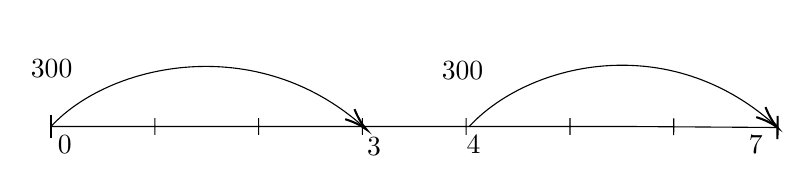
\begin{tikzpicture}[x=0.75pt,y=0.75pt,yscale=-1,xscale=1]
%uncomment if require: \path (0,301); %set diagram left start at 0, and has height of 301

%Straight Lines [id:da9438247164257243] 
\draw    (162,164.5) -- (336,164.5) -- (391,164.5) -- (438,164.5) -- (512,165) (212,160.5) -- (212,168.5)(262,160.5) -- (262,168.5)(312,160.5) -- (312,168.5)(362,160.5) -- (362,168.5)(412,160.5) -- (412,168.5)(462.03,160.66) -- (461.97,168.66)(512.03,161) -- (511.97,169) ;
\draw [shift={(512,165)}, rotate = 180.39] [color={rgb, 255:red, 0; green, 0; blue, 0 }  ][line width=0.75]    (0,5.59) -- (0,-5.59)   ;
\draw [shift={(162,164.5)}, rotate = 180] [color={rgb, 255:red, 0; green, 0; blue, 0 }  ][line width=0.75]    (0,5.59) -- (0,-5.59)   ;
%Curve Lines [id:da7543371493398257] 
\draw    (162,164.5) .. controls (189.86,134.15) and (261.28,118.16) .. (313.22,165.28) ;
\draw [shift={(314,166)}, rotate = 222.71] [color={rgb, 255:red, 0; green, 0; blue, 0 }  ][line width=0.75]    (10.93,-3.29) .. controls (6.95,-1.4) and (3.31,-0.3) .. (0,0) .. controls (3.31,0.3) and (6.95,1.4) .. (10.93,3.29)   ;
%Curve Lines [id:da026147367006871924] 
\draw    (363.5,164.5) .. controls (391.36,134.15) and (459.32,117.17) .. (511.22,164.28) ;
\draw [shift={(512,165)}, rotate = 222.71] [color={rgb, 255:red, 0; green, 0; blue, 0 }  ][line width=0.75]    (10.93,-3.29) .. controls (6.95,-1.4) and (3.31,-0.3) .. (0,0) .. controls (3.31,0.3) and (6.95,1.4) .. (10.93,3.29)   ;

% Text Node
\draw (164,167.5) node [anchor=north west][inner sep=0.75pt]   [align=left] {$\displaystyle 0$};
% Text Node
\draw (497,167.5) node [anchor=north west][inner sep=0.75pt]   [align=left] {$\displaystyle 7$};
% Text Node
\draw (313,168.5) node [anchor=north west][inner sep=0.75pt]   [align=left] {$\displaystyle 3$};
% Text Node
\draw (361,167.5) node [anchor=north west][inner sep=0.75pt]   [align=left] {$\displaystyle 4$};
% Text Node
\draw (151,131) node [anchor=north west][inner sep=0.75pt]   [align=left] {$\displaystyle 300$};
% Text Node
\draw (349,132) node [anchor=north west][inner sep=0.75pt]   [align=left] {$\displaystyle 300$};


\end{tikzpicture}
\end{center}
\begin{flalign*}
b) \; a(t) &= e ^{\integral{4}{7}{0.05 + 0.06s}{s}}&\\
&\;\;\vdots&
\end{flalign*}
\item Nos dan la siguiente fuerza de interés $\delta_t = \frac{2t}{1+t^2}$ encuentre la función de acumulación correspondiente.
\begin{flalign*}
&a(t) = e^{\integral{0}{t}{\frac{2t}{1+t^2}}{s}}& u = 1+s^2&\\
&\integral{0}{t}{\frac{25}{1+s^2}}{s} = - \int u^{-1}\, du = \ln\left(1+s^2 \right)\big|_0^t = \uline{\ln\left(1+t^2 \right) }  &du = 25ds&
\end{flalign*}
\item Encuentra el valor acumulado de $\$ 1,000$ invertido durante $10$ años a una tasa del $5\%$
\begin{flalign*}
&a(10) = e^{\delta_t(t)} = e^{10(0.05)}&\\
&\uline{A(10) = 1000e^{10(0.05)}}&
\end{flalign*}
\item Encuentre el valor acumulado de $\$500$ invertido durante $4$ años a una tasa del $2\%$

$A(4) = 500e^{4(0.02)} = \uline{541.6435}$
\item (Mal redactado)
\begin{align*}
&\delta_t = 0.05 + 0.01t, \; 0\leq t \leq 4&\\
&\$100(\text{son dos pagos})&
\end{align*}
\tikzset{every picture/.style={line width=0.75pt}} %set default line width to 0.75pt        
\begin{center}
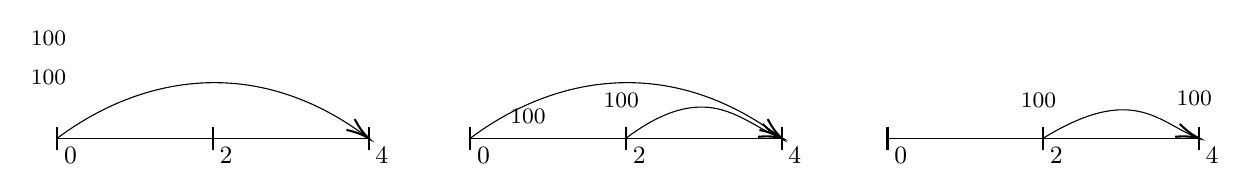
\begin{tikzpicture}[x=0.75pt,y=0.75pt,yscale=-1,xscale=1]
%uncomment if require: \path (0,300); %set diagram left start at 0, and has height of 300

%Straight Lines [id:da9622486181187222] 
\draw    (51,150.5) -- (201,150.5) ;
\draw [shift={(201,150.5)}, rotate = 180] [color={rgb, 255:red, 0; green, 0; blue, 0 }  ][line width=0.75]    (0,5.59) -- (0,-5.59)   ;
\draw [shift={(126,150.5)}, rotate = 180] [color={rgb, 255:red, 0; green, 0; blue, 0 }  ][line width=0.75]    (0,5.59) -- (0,-5.59)   ;
\draw [shift={(51,150.5)}, rotate = 180] [color={rgb, 255:red, 0; green, 0; blue, 0 }  ][line width=0.75]    (0,5.59) -- (0,-5.59)   ;
%Straight Lines [id:da02472881195252241] 
\draw    (250,150.5) -- (400,150.5) ;
\draw [shift={(400,150.5)}, rotate = 180] [color={rgb, 255:red, 0; green, 0; blue, 0 }  ][line width=0.75]    (0,5.59) -- (0,-5.59)   ;
\draw [shift={(325,150.5)}, rotate = 180] [color={rgb, 255:red, 0; green, 0; blue, 0 }  ][line width=0.75]    (0,5.59) -- (0,-5.59)   ;
\draw [shift={(250,150.5)}, rotate = 180] [color={rgb, 255:red, 0; green, 0; blue, 0 }  ][line width=0.75]    (0,5.59) -- (0,-5.59)   ;
%Straight Lines [id:da9609333128679138] 
\draw    (451,150.5) -- (601,150.5) ;
\draw [shift={(601,150.5)}, rotate = 180] [color={rgb, 255:red, 0; green, 0; blue, 0 }  ][line width=0.75]    (0,5.59) -- (0,-5.59)   ;
\draw [shift={(526,150.5)}, rotate = 180] [color={rgb, 255:red, 0; green, 0; blue, 0 }  ][line width=0.75]    (0,5.59) -- (0,-5.59)   ;
\draw [shift={(451,150.5)}, rotate = 180] [color={rgb, 255:red, 0; green, 0; blue, 0 }  ][line width=0.75]    (0,5.59) -- (0,-5.59)   ;
%Curve Lines [id:da7740865880763281] 
\draw    (51,150.5) .. controls (90.8,120.65) and (146.44,109.61) .. (200.19,149.89) ;
\draw [shift={(201,150.5)}, rotate = 217.21] [color={rgb, 255:red, 0; green, 0; blue, 0 }  ][line width=0.75]    (10.93,-3.29) .. controls (6.95,-1.4) and (3.31,-0.3) .. (0,0) .. controls (3.31,0.3) and (6.95,1.4) .. (10.93,3.29)   ;
%Curve Lines [id:da5017354164029006] 
\draw    (250,150.5) .. controls (289.8,120.65) and (345.44,109.61) .. (399.19,149.89) ;
\draw [shift={(400,150.5)}, rotate = 217.21] [color={rgb, 255:red, 0; green, 0; blue, 0 }  ][line width=0.75]    (10.93,-3.29) .. controls (6.95,-1.4) and (3.31,-0.3) .. (0,0) .. controls (3.31,0.3) and (6.95,1.4) .. (10.93,3.29)   ;
%Curve Lines [id:da48201812802025334] 
\draw    (325,150.5) .. controls (363.8,121.4) and (380.02,142.17) .. (398.3,149.83) ;
\draw [shift={(400,150.5)}, rotate = 200.22] [color={rgb, 255:red, 0; green, 0; blue, 0 }  ][line width=0.75]    (10.93,-3.29) .. controls (6.95,-1.4) and (3.31,-0.3) .. (0,0) .. controls (3.31,0.3) and (6.95,1.4) .. (10.93,3.29)   ;
%Curve Lines [id:da6855972323646] 
\draw    (526,150.5) .. controls (568.68,124.31) and (581.25,142.34) .. (599.31,149.84) ;
\draw [shift={(601,150.5)}, rotate = 200.22] [color={rgb, 255:red, 0; green, 0; blue, 0 }  ][line width=0.75]    (10.93,-3.29) .. controls (6.95,-1.4) and (3.31,-0.3) .. (0,0) .. controls (3.31,0.3) and (6.95,1.4) .. (10.93,3.29)   ;

% Text Node
\draw (53,153.5) node [anchor=north west][inner sep=0.75pt]  [font=\small] [align=left] {$\displaystyle 0$};
% Text Node
\draw (203,153.5) node [anchor=north west][inner sep=0.75pt]  [font=\small] [align=left] {$\displaystyle 4$};
% Text Node
\draw (252,153.5) node [anchor=north west][inner sep=0.75pt]  [font=\small] [align=left] {$\displaystyle 0$};
% Text Node
\draw (402,153.5) node [anchor=north west][inner sep=0.75pt]  [font=\small] [align=left] {$\displaystyle 4$};
% Text Node
\draw (603,153.5) node [anchor=north west][inner sep=0.75pt]  [font=\small] [align=left] {$\displaystyle 4$};
% Text Node
\draw (453,153.5) node [anchor=north west][inner sep=0.75pt]  [font=\small] [align=left] {$\displaystyle 0$};
% Text Node
\draw (128,153.5) node [anchor=north west][inner sep=0.75pt]  [font=\small] [align=left] {$\displaystyle 2$};
% Text Node
\draw (327,153.5) node [anchor=north west][inner sep=0.75pt]  [font=\small] [align=left] {$\displaystyle 2$};
% Text Node
\draw (528,153.5) node [anchor=north west][inner sep=0.75pt]  [font=\small] [align=left] {$\displaystyle 2$};
% Text Node
\draw (37,116.5) node [anchor=north west][inner sep=0.75pt]  [font=\footnotesize] [align=left] {$\displaystyle 100$};
% Text Node
\draw (37,97.5) node [anchor=north west][inner sep=0.75pt]  [font=\footnotesize] [align=left] {$\displaystyle 100$};
% Text Node
\draw (268,135.5) node [anchor=north west][inner sep=0.75pt]  [font=\footnotesize] [align=left] {$\displaystyle 100$};
% Text Node
\draw (313,127.5) node [anchor=north west][inner sep=0.75pt]  [font=\footnotesize] [align=left] {$\displaystyle 100$};
% Text Node
\draw (514,127.5) node [anchor=north west][inner sep=0.75pt]  [font=\footnotesize] [align=left] {$\displaystyle 100$};
% Text Node
\draw (589,126.5) node [anchor=north west][inner sep=0.75pt]  [font=\footnotesize] [align=left] {$\displaystyle 100$};


\end{tikzpicture}
\end{center}
\begin{flalign*}
&a(t) = e^{\integral{0}{t}{\delta_s}{s}} = e^{\integral{0}{4}{0.05+0.01s}{s}} = e^{0.05s\big|_0^4 - \frac{0.01}{2}s^2\big|_0^4}=(*)&\\
&\hfill &\\
&\text{a)} \: \Longrightarrow \: A(4) = 200(*) \, \text{si los 2 pagos en t=0}&\\
&\text{b)} \: \Longrightarrow \: A(4) = 100(*) + 100e^{\integral{2}{4}{\delta_s}{s}}&\\
&\text{c)} \: \Longrightarrow \: A(4) = 100e^{\integral{2}{4}{\delta_s}{s}} +100&
\end{flalign*}
\end{enumerate}

$V_a(t) = \frac{1}{a(t)} \: \longrightarrow \:$ Función valor presente.
$$\underbrace{\delta_{t^{*}}}_{ \text{Fuerza de descuento}} = \frac{-\dpartial{t}V_a(t)}{V_a(t)} \hspace{2cm} \delta_t^* = \underbrace{\delta_t}_{\text{Fuerza de interés}}$$

\begin{theorem}
\begin{flalign*}
&V_a(t) = 1-td&\\
&V_a(t) = (1-d)^{t}&
\end{flalign*}
\end{theorem}
\begin{lemma}
Para $\alpha \in \RR \: \lim_{m \to \infty} \left(1 + \frac{\alpha}{m} \right)^{m} = e^{\alpha} $ 
\end{lemma}
\begin{proof}
\begin{align*}
&\lim_{m\to\infty} \left(1 + \frac{\alpha}{m} \right)^m =  \lim_{m\to\infty} e^{m\log\left(1 + \frac{\alpha}{m} \right)} \: \ldots \: (1)&\\
&\text{y además}&\\
&\lim_{m\to\infty}m\log\left(1 +\frac{\alpha}{m} \right) = \lim_{m\to\infty}\frac{\log\left(1 +\frac{\alpha}{m} \right)}{\frac{1}{m}} \mathrel{\stackon[1pt]{$=$}{$\scriptscriptstyle \text{L'Hôpital}$}}     \lim_{m \to \infty} \frac{\frac{1}{1+\frac{\alpha}{m}}\left(\frac{-\alpha}{m^2} \right) }{-\frac{1}{m^2}}&\\
&\lim_{m \to \infty} \frac{\alpha}{1+\frac{\alpha}{m}} = \frac{\alpha}{1} \: \Longrightarrow \: \lim_{m\to\infty} m\log\left( 1 +\frac{\alpha}{m}\right) = \alpha &\\
&\Longrightarrow \: \exp{\left\lbrace\lim_{m\to\infty}m\log\left( 1 + \frac{\alpha}{m}\right)  \right\rbrace } = e^{\alpha} \: \Longrightarrow \: \lim_{m\to\infty}\exp{\left\lbrace m\log\left( 1 + \frac{\alpha}{m}\right)  \right\rbrace } = e^{\alpha}&\\
&(\text{pues}\, e^t \, \text{es absolutamente continua})&
\end{align*}
\end{proof}
\begin{proposition}
Si $i^{(m)} \sim \delta$ entonces $\lim_{m\to\infty} i^{(m)} = \delta$
\end{proposition}
\begin{proof}
Como $i^{(m)} \sim \delta$ entonces 
\begin{align*}
&\left(1 + \frac{i^{(m)}}{m} \right)^m = e^{\delta} \: \Longrightarrow \: \lim_{m\to\infty} \left( 1 + \frac{i^{(m)}}{m}\right)^m = e^{\delta}\\
& \Longrightarrow \: e^{i^{(m)}} = e^{\delta}\\
& \therefore \: i^{(m)} \mathrel{\stackon[1pt]{$\longrightarrow $}{$\scriptscriptstyle m\rightarrow \infty$}} \delta      
\end{align*}
\end{proof}
\begin{center}
\tikzset{every picture/.style={line width=0.75pt}} %set default line width to 0.75pt        

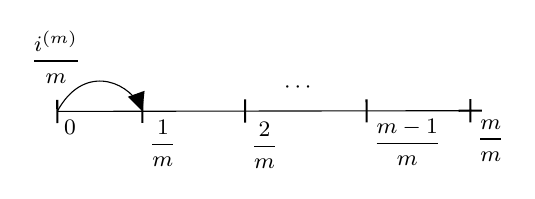
\begin{tikzpicture}[x=0.75pt,y=0.75pt,yscale=-1,xscale=1]
%uncomment if require: \path (0,300); %set diagram left start at 0, and has height of 300

%Straight Lines [id:da36963066609877826] 
\draw    (251,150.67) -- (333,150.53) -- (350,150.5) -- (450,150.33) ;
\draw [shift={(450,150.33)}, rotate = 359.9] [color={rgb, 255:red, 0; green, 0; blue, 0 }  ][line width=0.75]    (-5.59,0) -- (5.59,0)(0,5.59) -- (0,-5.59)   ;
\draw [shift={(292,150.6)}, rotate = 539.9] [color={rgb, 255:red, 0; green, 0; blue, 0 }  ][line width=0.75]    (0,5.59) -- (0,-5.59)   ;
\draw [shift={(341.5,150.52)}, rotate = 539.9] [color={rgb, 255:red, 0; green, 0; blue, 0 }  ][line width=0.75]    (0,5.59) -- (0,-5.59)   ;
\draw [shift={(400,150.41)}, rotate = 539.9] [color={rgb, 255:red, 0; green, 0; blue, 0 }  ][line width=0.75]    (0,5.59) -- (0,-5.59)   ;
\draw [shift={(251,150.67)}, rotate = 539.9] [color={rgb, 255:red, 0; green, 0; blue, 0 }  ][line width=0.75]    (0,5.59) -- (0,-5.59)   ;
%Curve Lines [id:da17595121368939615] 
\draw    (251,150.67) .. controls (263.16,128.07) and (284.05,135.34) .. (290.8,147.91) ;
\draw [shift={(292,150.6)}, rotate = 250.48000000000002] [fill={rgb, 255:red, 0; green, 0; blue, 0 }  ][line width=0.08]  [draw opacity=0] (8.93,-4.29) -- (0,0) -- (8.93,4.29) -- cycle    ;

% Text Node
\draw (253,153.67) node [anchor=north west][inner sep=0.75pt]  [font=\footnotesize] [align=left] {$\displaystyle 0$};
% Text Node
\draw (294,153.6) node [anchor=north west][inner sep=0.75pt]  [font=\footnotesize] [align=left] {$\displaystyle \frac{1}{m}$};
% Text Node
\draw (343,154.6) node [anchor=north west][inner sep=0.75pt]  [font=\footnotesize] [align=left] {$\displaystyle \frac{2}{m}$};
% Text Node
\draw (402,153.41) node [anchor=north west][inner sep=0.75pt]  [font=\footnotesize] [align=left] {$\displaystyle \frac{m-1}{m}$};
% Text Node
\draw (452,153.33) node [anchor=north west][inner sep=0.75pt]  [font=\footnotesize] [align=left] {$\displaystyle \frac{m}{m}$};
% Text Node
\draw (359,135.6) node [anchor=north west][inner sep=0.75pt]  [font=\footnotesize] [align=left] {$\displaystyle \cdots $};
% Text Node
\draw (237,110.6) node [anchor=north west][inner sep=0.75pt]  [font=\footnotesize] [align=left] {$\displaystyle \frac{i^{( m)}}{m}$};
\end{tikzpicture}
\end{center}

Cuando $m$ es grande estas particiones son chiquitas.

En ese caso límite movernos con la tasa nominal es equivalente a movernos con la fuerza de interés.

En la práctica es muy común hacer $i^{(365)}\approx \delta$

\begin{lemma}
Si $c>0$, entonces la función \uline{$g(x) = x\left[(1+c)^{1/x} -1\right] $} es decreciente.
\end{lemma}
\begin{proposition}
Si $i\sim i^{(2)} \sim i^{(4)} \sim i^{(12)} \sim i^{(360)}$ entonces $i^{(360)}<i^{(12)}<i^{(6)}<i$
\end{proposition}
\begin{proof}
Como $i\sim i^{(m)} \: \Rightarrow \: 1+i = \left( 1 + \frac{i^{(m)}}{m}\right)^{m} \: \Rightarrow \: i^{(m)} = m \left[(1+i)^{1/m}-1\right]  $
\begin{align*}
&\text{Nótese que}&\\
&1<2<3<\ldots<360&\\
&\mathrel{\stackon[1pt]{$\Longrightarrow$}{$\scriptscriptstyle \text{Lema}$}} \: g(1)>g(2)>\ldots>g(360)&\\
&\Longrightarrow \: 1\left[(1+c)^{1/1} -1\right]>\ldots>360\left[(1+c)^{1/360}-1 \right]&\\
&\text{En partícular si}\, c=i:\\
&1\left[(1+i)^{1/1}-1 \right]>\ldots>360\left[(1+c)^{1/360}-1 \right] \: \Longrightarrow \: i>i^{(2)}>i^{(3)}>\ldots>i^{(360)}&   
\end{align*}
\end{proof}
\begin{proposition}
Si $d\sim d^{(2)}\sim \, \ldots \, \sim d^{(360)}$ entonces $d<d^{(2)}<\,\ldots \, <d^{(360)}$
\end{proposition}
Ya con todas estas proposiciones, si $d\sim d^{(2)}\sim \, \ldots \, \sim d^{(360)} \sim \delta \sim i^{(360)} \sim \, \ldots \, \sim i$, entonces $d<d^{(2)}<\ldots<d^{(360)} < \delta < i^{(360)}<\ldots<i$.
\begin{lemma}
Para cualquier $c>0$
\begin{enumerate}
\item[(1)] Si $t\in(0,1)$, entonces $1+ct > (1+c)^t$
\item[(2)] Si $t>1$, entonces $1+ct < (1+c)^t$
\item[(3)] Si $t=1$, entonces $1+ct = (1+c)^t$
\end{enumerate}
\end{lemma}
\begin{proof}
Si $c\in [0,1)$

Considérese la función $f(c) = (1+c)^t$

El polinomio de Taylor de $f$ alrededor de $c^*=0$ es $f(c) = \sum_{k=0}^{\infty} \frac{f^{(k)}(0)}{k!}(c-0)^k \: \ldots \: (\#)$

Sin embargo 
\begin{align*}
f'(c) &= t(1+c)^{t-1}&\\
f''(c) &= t(t-1)(1+c)^{t-i}&\\
\Longrightarrow \: &f'(0) = t&\\
\Longrightarrow \: &f''(0) = t(t-1)&\\
& f(0) = 1&\\
&\vdots&\\
&f^{(k)}(c) = t(t-1) \cdots (t-k+1)(1+c)^{t-k}&\\
\Longrightarrow &f^{(k)} = t(t-1)\cdots (t-k+1)&
\end{align*}
Regresando a $(\#)$
\begin{align*}
&f(c) = \frac{1}{0!}c^0 + \frac{t}{1}c^1 + \frac{t(t-1)}{2}c^2 + \frac{t(t-1)(t-2)}{3!}c^3 + \: \ldots \: + \frac{t(t-1)\: \cdots  \: (t-k+1)}{k!}c^k + \cdots\\
&=1+tc + (t-1)\left[\frac{tc^2}{2}+ \frac{t(t-2)c^3}{3!} + \: \cdots \: + \frac{t(t-2) \: \cdots \: (t-k+1)c^k}{k!}+ \: \ldots \:\right] 
\end{align*}
Concluimos que $(1+c)^t \boxed{\mathrel{\stackon[1pt]{$\mathrel{\stackon[1pt]{$\scriptstyle=$}{$\scriptstyle<$}}$}{$\scriptstyle>$}}} 1+ct+(t-1)\beta$, donde $\beta \approx 0$
\medskip

$\cdot$ Si $t>1$: $\: (1+c)^t > 1+ct$

$\cdot$ Si $t<1$: $\: (1+c)^t < 1+ct$

En particular si $c=i$

\setulcolor{red}\ul{$(1+i)^t > 1+it, \, \text{si} \, t>1$}

Para periodos mayores a $1$, el interés compuesto le gana al interés simple.

\setulcolor{red}\ul{$(1+i)^t < 1+it$}, si $t<1$

Para periodos menores a 1 el interés simple le gana al compuesto
\end{proof}

\uline{\uline{Tasa manda}}

\uline{Notación}
\begin{itemize}
\item[$\cdot$] Cuando no especifica $a(\cdot)$ y solo se da una tasa de interés $i$ se supone $a(t) = (1+i)^t$ (compuesto).
\item[$\cdot$] Para el caso de interés compuesto se denota como $\color{red}\boxed{\color{black} V:= \frac{1}{1+i}}$

Algunos libros ocupan: $V_i := \frac{1}{1+i}$

\item[-] A \textcolor{blue}{\uline{$V$}} se le conoce como \textcolor{blue}{\uline{factor de descuento.}}

\item[-]A \textcolor{blue}{\uline{$(1+i)$}} se le conoce como \textcolor{blue}{\uline{factor de acumulación.}}
\end{itemize}

\begin{proposition}
Si $i\sim d$, entonces:
\begin{enumerate}
\item[(1)] \setulcolor{red}\ul{$d = iv$}
\item[(2)] \setulcolor{red}\ul{$d = 1-v$}
\end{enumerate}
\end{proposition}
\begin{proof}
\begin{align*}
(2) \quad i\sim d \: &\Longrightarrow \: (1+i) = (1-d)^{-1} \\
& \Longrightarrow \: \frac{1}{1+i} = 1-d \: \Longrightarrow \: V = 1-d \: \Longrightarrow \: d=1-V \; \boxed{}\\
&\hfill \\
(1) \hspace{1.3cm} &(1+i) = (1-d)^{-1} \\
& \Longrightarrow \: \frac{1}{1+i} = 1-d \: \Longrightarrow \: d = 1 - \frac{1}{1+i} = \frac{1+i-1}{1+i} = \frac{i}{1+i} = i\frac{1}{1+i} = iV\\
& \therefore \: d=iV \: \boxed{}
\end{align*}
\end{proof}
\uline{Recordar}
\begin{itemize}
\item[$\cdot$] $i\sim d \sim i^{(m)} \sim d^{(p)} \sim \delta$ si 

$(1+i) = (1-d)^{-1} = \left(1+ \frac{i^{(m)}}{m} \right)^m = e^{\delta} = \left(1 - \frac{d^{(p)}}{p} \right)^{-p}$
\item[$\cdot$] $a(t) = (1+i)^t = V^{-t}\\
V_a(t) = \frac{1}{a(t)} = \frac{1}{(1+i)^t} = V^t$
\end{itemize}

\begin{remark}
\begin{align*}
&\prod_{k=1}^{n} \left(1 + i_k \right) = \prod_{k=1}^{n} \left(1 + \frac{a(k) - a(k-1)}{a(k-1)} \right) = \prod_{k=1}^{n} \left(\frac{\cancel{a(k-1)} + a(k) - \cancel{a(k-1)}}{a(k-1)} \right)&\\
&= \prod_{k=1}^{n} \frac{a(k)}{a(k-1)} = \frac{a(1)}{a(0)} \cdot \frac{(2)}{a(1)} \cdot \: \ldots \: \cdot \frac{a(n)}{a(n-1)} = \frac{a(n)}{a(0)} = a(n)&
\end{align*}
$$ \therefore \: \color{blue}\boxed{\color{black} a(n) = \prod_{k=1}^{n} \left( 1+i_k\right) }$$
\begin{align*}
&\text{También} \quad \prod_{k=1}^{n}\left(1-d_k \right) = \prod_{k=1}^{n} \left(1 - \frac{a(k) -a(k-1)}{a(k)}\right) = \prod_{k=1}^{n} \left(\frac{\cancel{a(k)} - \cancel{a(k)} + a(k-1)}{a(k)} \right)   &\\
&= \prod_{k=1}^{n} \frac{a(k-1)}{a(k)}= \frac{a(0)}{a(1)} \cdot \frac{a(1)}{a(2)} \: \cdots \: \frac{a(n-1)}{a(n)} = \frac{a(0)}{a(n)} = \frac{1}{a(n)} = V_a(n)&
\end{align*}
$$\color{blue}\boxed{\color{black}V_a(n)=\prod_{k=1}^{n} (1-d_k)} \hspace{0.5cm} \color{black}\text{ó equivalentemente} \hspace{0.5cm} \color{blue}\boxed{\color{black}a(n)=\prod_{k=1}^{n} -(1-d_k)^{-1}}$$
\end{remark}

También ocurre las relaciones entre $a(t)$ y $\delta_t \: \ldots$ 
$$\delta_t = \frac{a'(t)}{a(t)} = \dpartial{t} \log\left( a(t) \right) \hspace{0.5cm} \therefore \: a(t) = e^{\integral{0}{t}{\delta_s}{s}}$$

$\cdot \quad \text{Sean} \: 0<t_1<t_2$
\begin{align*}
&\text{Sabemos que} \, a(t_2) = \exp\left\lbrace \integral{0}{t_2}{\delta_s}{s} \right\rbrace = \exp\left\lbrace \integral{0}{t_1}{\delta_s}{s} + \integral{t_1}{t_2}{\delta_s}{s} \right\rbrace &\\
&=\exp\left\lbrace \integral{0}{t_1}{\delta_s}{s}\right\rbrace \cdot \exp\left\lbrace \integral{t_1}{t_2}{\delta_s}{s} \right\rbrace = a(t_1)\exp\left\lbrace \integral{t_1}{t_2}{\delta_s}{s}\right\rbrace &\\
&\Longrightarrow \: \frac{a(t_2)}{a(t_1)} = \exp\left\lbrace \integral{t_1}{t_2}{\delta_s}{s}\right\rbrace \: \ldots \: (\MakeUppercase{\romannumeral 2})&
\end{align*}

$(\MakeUppercase{\romannumeral 2})$ sirve en los casos en los que una inversión \textcolor{blue}{no empieza en 0 si no en $t_1$ y termina en $t_2$}

\begin{center}
\tikzset{every picture/.style={line width=0.75pt}} %set default line width to 0.75pt        

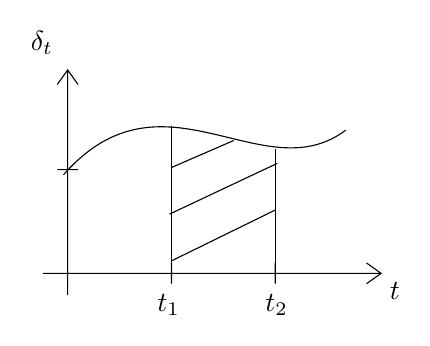
\begin{tikzpicture}[x=0.75pt,y=0.75pt,yscale=-1,xscale=1]
%uncomment if require: \path (0,300); %set diagram left start at 0, and has height of 300

%Shape: Axis 2D [id:dp7771223720940366] 
\draw  (289,201.5) -- (452,201.5)(301,103.5) -- (301,212) (445,196.5) -- (452,201.5) -- (445,206.5) (296,110.5) -- (301,103.5) -- (306,110.5) (351,196.5) -- (351,206.5)(401,196.5) -- (401,206.5)(296,151.5) -- (306,151.5) ;
\draw   ;
%Curve Lines [id:da1275936857163802] 
\draw    (299,154) .. controls (347,99.5) and (395,162.5) .. (435,132.5) ;
%Straight Lines [id:da7557150443518144] 
\draw    (351,130.5) -- (351,201.5) ;
%Straight Lines [id:da5694519936840394] 
\draw    (401,141.5) -- (401,200.5) ;
%Straight Lines [id:da32445376790004476] 
\draw    (350,173) -- (402,148.5) ;
%Straight Lines [id:da3400339103900818] 
\draw    (351,195.5) -- (401,171) ;
%Straight Lines [id:da5904754511535812] 
\draw    (351,150.5) -- (381,137.5) ;

% Text Node
\draw (343,210.4) node [anchor=north west][inner sep=0.75pt]    {$t_{1}$};
% Text Node
\draw (395,210.4) node [anchor=north west][inner sep=0.75pt]    {$t_{2}$};
% Text Node
\draw (455,204.4) node [anchor=north west][inner sep=0.75pt]    {$t$};
% Text Node
\draw (282,83.4) node [anchor=north west][inner sep=0.75pt]    {$\delta _{t}$};


\end{tikzpicture}
\end{center}

También, de la relación entre $a(t)$ y $\delta_t$
\begin{align*}
&a(t) = \exp\left\lbrace \integral{0}{t}{\delta_s}{s} \right\rbrace \\
& \Longrightarrow \frac{1}{a(t)} = \exp\left\lbrace - \integral{0}{t}{\delta_t}{s}\right\rbrace \\
&\color{blue}\boxed{\color{black}\therefore \: V_a(t) = \exp\left\lbrace - \integral{0}{t}{\delta_s}{s} \right\rbrace}
\end{align*}

\textcolor{blue}{Interpretación económica de los modelos de descuento}

Supóngase que un banco le presta una cantidad $M$, pero le cobra por adelantado los intereses en una porción $c$ por cada peso prestado por cada periodo de préstamo.

¿Si yo pido prestado a $n$ periodos cuánto recibiré hoy?
\begin{itemize}
\item[$\cdot$] Si yo pido a 1 periodo, recibiré $M-Mc = \uline{M(1-c)}$
\item[$\cdot$] Si yo pido a 2 periodos, recibiré $M(1-c) - M(1-c)c = M(1-c)(1-c) = \uline{M(1-c)^2}$
\item[$\cdot$] Si yo pido a 2 periodos, recibiré $M(1-c)^2 - M(1-c)^2 \cdot c = M(1-c)^2[1-c] = \uline{M(1-c)^3}$
\end{itemize}
Inductivamente, si yo pido a $n$ periodos, recibiré $\color{red}\boxed{\color{black}M(1-c)^n}$

Si $d=c$ nos recuerda al descuento compuesto $V_a(t) = (1-d)^t$ 

\color{red}\circled{Tarea: } Interpretación del descuento simple.\color{black}

\begin{proposition}
Si $d^{(p)} \sim \delta$, entonces $\color{blue}\boxed{\color{black} \lim_{p \to \infty} d^{(p)} = \delta }$
\end{proposition}
\begin{proof}
Anteriormente probamos que $\forall \: \alpha \in \RR \; \lim_{n \to \infty} \left(1 + \frac{\alpha}{n} \right)^n = e^{\alpha}$
\begin{align*}
&\lim_{p \to \infty} \left(1 - \frac{d^{(p)}}{p} \right)^p = \lim_{p \to \infty} \left(1 + \frac{-d^{(p)}}{p} \right)^p = e^{-d^{(p)}} \\
&\text{Sin embargo} \, d^{(p)} \sim \delta \\
&\left(1 - \frac{d^{(p)}}{p} \right)^{-p} = e^{\delta} \: \Longrightarrow \: \lim_{p \to \infty} \left(1+ \frac{-d^{(p)}}{p} \right)^{-p} = e^{\delta} \: \Longrightarrow \: \left(1 - \frac{d^{(p)}}{p}\right)^{-p} = e^{-\delta}\\
&\text{Entonces} \\
& - d^{(p)} \mathrel{\stackon[1pt]{$\longrightarrow $}{$\scriptscriptstyle p\rightarrow \infty$}} -\delta \\
& \hspace{0.5cm} d^{(p)} \mathrel{\stackon[1pt]{$\longrightarrow $}{$\scriptscriptstyle p\rightarrow \infty$}} \delta 
\end{align*}
\end{proof}
\begin{lemma}
Considérese la función $\boxed{h(x) := x\left[ 1-(1-c)^{1/x}\right] }$, entonces $x \longmapsto h(x)$  es \uline{creciente}.
\end{lemma}
Objetivo: demostrar que $d<d^{(2)}<d^{(3)}<\ldots<d^{(360)}<\delta$
\begin{proof}
Como $1<2<3<\ldots<360$

Según el lema $h(1)<h(2)<h(3)<\ldots<h(360)$
\begin{align*}
&\Longrightarrow 1\left[ 1-(1-c)^{1/1}\right] < 2\left[ 1-(1-c)^{1/2}\right] < \ldots < 360\left[ 1-(1-c)^{1/360}\right]&\\
&\text{Si} \, d=c &\\
&\Longrightarrow 1\left[ 1-(1-d)^{1/1}\right] < 2\left[ 1-(1-d)^{1/2}\right] < \ldots < 360\left[ 1-(1-d)^{1/360}\right]&\\
&\therefore \: d<d^{(2)}<\ldots<d^{(360)}&
\end{align*}
\end{proof}
\textbf{Ayudantía}

\textbf{Ejemplo: }
\begin{center}
\tikzset{every picture/.style={line width=0.75pt}} %set default line width to 0.75pt        
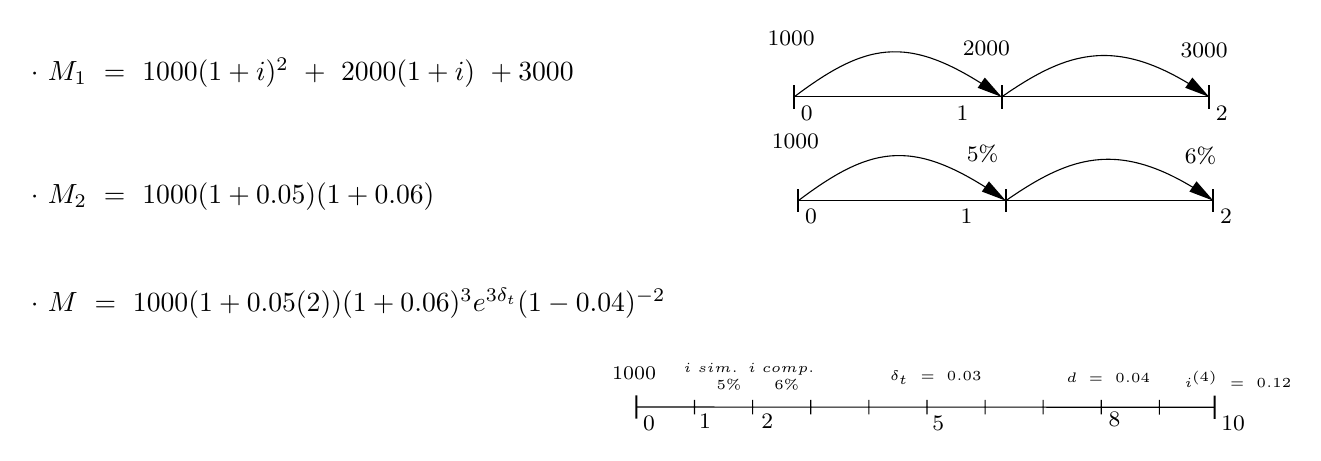
\begin{tikzpicture}[x=0.75pt,y=0.75pt,yscale=-1,xscale=1]
%uncomment if require: \path (0,300); %set diagram left start at 0, and has height of 300

%Straight Lines [id:da27736570369124625] 
\draw    (373,150.5) -- (573,150.5) ;
\draw [shift={(573,150.5)}, rotate = 180] [color={rgb, 255:red, 0; green, 0; blue, 0 }  ][line width=0.75]    (0,5.59) -- (0,-5.59)   ;
\draw [shift={(473,150.5)}, rotate = 180] [color={rgb, 255:red, 0; green, 0; blue, 0 }  ][line width=0.75]    (0,5.59) -- (0,-5.59)   ;
\draw [shift={(373,150.5)}, rotate = 180] [color={rgb, 255:red, 0; green, 0; blue, 0 }  ][line width=0.75]    (0,5.59) -- (0,-5.59)   ;
%Curve Lines [id:da10604097932862588] 
\draw    (373,150.5) .. controls (409.63,122.78) and (429.6,120.54) .. (471.72,149.61) ;
\draw [shift={(473,150.5)}, rotate = 214.9] [fill={rgb, 255:red, 0; green, 0; blue, 0 }  ][line width=0.08]  [draw opacity=0] (12,-3) -- (0,0) -- (12,3) -- cycle    ;
%Curve Lines [id:da7758527522575427] 
\draw    (473,150.5) .. controls (505.67,127.73) and (529.52,120.64) .. (571.72,149.61) ;
\draw [shift={(573,150.5)}, rotate = 214.9] [fill={rgb, 255:red, 0; green, 0; blue, 0 }  ][line width=0.08]  [draw opacity=0] (12,-3) -- (0,0) -- (12,3) -- cycle    ;
%Straight Lines [id:da9555752261431487] 
\draw    (295,249.9) -- (573.63,250.02) (323,246.42) -- (323,253.42)(351,246.43) -- (351,253.43)(379,246.44) -- (379,253.44)(407,246.45) -- (407,253.45)(435,246.46) -- (435,253.46)(463,246.48) -- (463,253.48)(491,246.49) -- (491,253.49)(519,246.5) -- (519,253.5)(547,246.51) -- (547,253.51) ;
\draw [shift={(573.63,250.02)}, rotate = 180.02] [color={rgb, 255:red, 0; green, 0; blue, 0 }  ][line width=0.75]    (0,5.59) -- (0,-5.59)   ;
\draw [shift={(295,249.9)}, rotate = 180.02] [color={rgb, 255:red, 0; green, 0; blue, 0 }  ][line width=0.75]    (0,5.59) -- (0,-5.59)   ;
%Straight Lines [id:da9930737794402731] 
\draw    (371,100.5) -- (571,100.5) ;
\draw [shift={(571,100.5)}, rotate = 180] [color={rgb, 255:red, 0; green, 0; blue, 0 }  ][line width=0.75]    (0,5.59) -- (0,-5.59)   ;
\draw [shift={(471,100.5)}, rotate = 180] [color={rgb, 255:red, 0; green, 0; blue, 0 }  ][line width=0.75]    (0,5.59) -- (0,-5.59)   ;
\draw [shift={(371,100.5)}, rotate = 180] [color={rgb, 255:red, 0; green, 0; blue, 0 }  ][line width=0.75]    (0,5.59) -- (0,-5.59)   ;
%Curve Lines [id:da2201481465694839] 
\draw    (371,100.5) .. controls (407.63,72.78) and (427.6,70.54) .. (469.72,99.61) ;
\draw [shift={(471,100.5)}, rotate = 214.9] [fill={rgb, 255:red, 0; green, 0; blue, 0 }  ][line width=0.08]  [draw opacity=0] (12,-3) -- (0,0) -- (12,3) -- cycle    ;
%Curve Lines [id:da29027599663516246] 
\draw    (471,100.5) .. controls (503.67,77.73) and (527.52,70.64) .. (569.72,99.61) ;
\draw [shift={(571,100.5)}, rotate = 214.9] [fill={rgb, 255:red, 0; green, 0; blue, 0 }  ][line width=0.08]  [draw opacity=0] (12,-3) -- (0,0) -- (12,3) -- cycle    ;

% Text Node
\draw (2,80.4) node [anchor=north west][inner sep=0.75pt]    {$\cdot \ M_{1} \ =\ 1000( 1+i)^{2} \ +\ 2000( 1+i) \ +3000$};
% Text Node
\draw (2,140.4) node [anchor=north west][inner sep=0.75pt]    {$\cdot \ M_{2} \ =\ 1000( 1+0.05)( 1+0.06)$};
% Text Node
\draw (2,191.4) node [anchor=north west][inner sep=0.75pt]    {$\cdot \ M \ =\ 1000( 1+0.05( 2))( 1+0.06)^{3} e^{3\delta _{t}}( 1-0.04)^{-2}$};
% Text Node
\draw (575,153.5) node [anchor=north west][inner sep=0.75pt]  [font=\footnotesize] [align=left] {$\displaystyle 2$};
% Text Node
\draw (359,117.4) node [anchor=north west][inner sep=0.75pt]  [font=\footnotesize]  {$1000$};
% Text Node
\draw (453,122.4) node [anchor=north west][inner sep=0.75pt]  [font=\footnotesize]  {$5\%$};
% Text Node
\draw (558,123.4) node [anchor=north west][inner sep=0.75pt]  [font=\footnotesize]  {$6\%$};
% Text Node
\draw (297,252.9) node [anchor=north west][inner sep=0.75pt]  [font=\footnotesize] [align=left] {$\displaystyle 0$};
% Text Node
\draw (575.63,253.02) node [anchor=north west][inner sep=0.75pt]  [font=\footnotesize] [align=left] {$\displaystyle 10$};
% Text Node
\draw (375,153.5) node [anchor=north west][inner sep=0.75pt]  [font=\footnotesize] [align=left] {$\displaystyle 0$};
% Text Node
\draw (450,153.5) node [anchor=north west][inner sep=0.75pt]  [font=\footnotesize] [align=left] {$\displaystyle 1$};
% Text Node
\draw (324,252) node [anchor=north west][inner sep=0.75pt]  [font=\footnotesize] [align=left] {1};
% Text Node
\draw (354,252) node [anchor=north west][inner sep=0.75pt]  [font=\footnotesize] [align=left] {2};
% Text Node
\draw (436.32,252.96) node [anchor=north west][inner sep=0.75pt]  [font=\footnotesize] [align=left] {5};
% Text Node
\draw (521.32,251) node [anchor=north west][inner sep=0.75pt]  [font=\footnotesize] [align=left] {8};
% Text Node
\draw (282,229.4) node [anchor=north west][inner sep=0.75pt]  [font=\scriptsize]  {$1000$};
% Text Node
\draw (310,226.4) node [anchor=north west][inner sep=0.75pt]  [font=\tiny]  {$ \begin{array}{l}
i\ sim.\\
\ \ \ \ \ 5\%
\end{array}$};
% Text Node
\draw (341,226.4) node [anchor=north west][inner sep=0.75pt]  [font=\tiny]  {$ \begin{array}{l}
i\ comp.\\
\ \ \ \ 6\%
\end{array}$};
% Text Node
\draw (416,231.4) node [anchor=north west][inner sep=0.75pt]  [font=\tiny]  {$\delta _{t} \ =\ 0.03$};
% Text Node
\draw (501,232.4) node [anchor=north west][inner sep=0.75pt]  [font=\tiny]  {$d\ =\ 0.04$};
% Text Node
\draw (558,231.4) node [anchor=north west][inner sep=0.75pt]  [font=\tiny]  {$i^{( 4)} \ =\ 0.12$};
% Text Node
\draw (573,103.5) node [anchor=north west][inner sep=0.75pt]  [font=\footnotesize] [align=left] {$\displaystyle 2$};
% Text Node
\draw (357,67.4) node [anchor=north west][inner sep=0.75pt]  [font=\footnotesize]  {$1000$};
% Text Node
\draw (451,72.4) node [anchor=north west][inner sep=0.75pt]  [font=\footnotesize]  {$2000$};
% Text Node
\draw (556,73.4) node [anchor=north west][inner sep=0.75pt]  [font=\footnotesize]  {$3000$};
% Text Node
\draw (373,103.5) node [anchor=north west][inner sep=0.75pt]  [font=\footnotesize] [align=left] {$\displaystyle 0$};
% Text Node
\draw (448,103.5) node [anchor=north west][inner sep=0.75pt]  [font=\footnotesize] [align=left] {$\displaystyle 1$};
\end{tikzpicture}
\end{center}

\color{blue}
\begin{itemize}
\item[*] $d$ se hace al inicio del periodo
\item[*] $i$ al final del periodo
\end{itemize}
\color{black}
\uline{De la tarea:}
\begin{itemize}
\item[\circled{13}] $i$ simple = $11\%$

$d$ simple
\item[$\cdot$] $(1+0.11) = \frac{1}{1-dt} = \left( 1 -d(1)\right)^{-1} = \underbrace{(1-d)^{-1}}_{\text{1 año }} $
\item[$\cdot$] $\left( 1+0.11\left(\frac{1}{2} \right) \right)  = \underbrace{\left(1-d\left(\frac{1}{2} \right)  \right)^{-1}}_{\text{6 meses}} $
\item[\circled{30}] $1980 = M_a( \mathrel{\stackon[1.5pt]{$7$}{$k^{(2)}$}})a(\mathrel{\stackon[1.5pt]{$3.5$}{$k^{(4)}$}})$

$\therefore \: 1000\left( 1 + \frac{k^{(2)}}{2}\right)^{2(7)} \left(1 + 2\frac{k^{(4)}}{4} \right)^{4(3.5)}  $
\end{itemize}
\newpage
\color{blue}\boxed{$\color{black}\text{Dudas}$}
\color{black}
\begin{enumerate}[label=\protect\circled{\arabic*}]
\item ¿Qué pasa si tengo varias funciones de acumulación para una misma inversión?
\begin{center}
\tikzset{every picture/.style={line width=0.75pt}} %set default line width to 0.75pt        
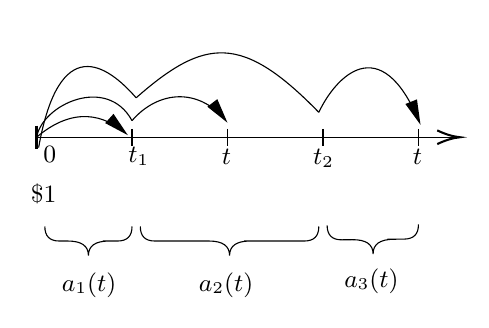
\begin{tikzpicture}[x=0.75pt,y=0.75pt,yscale=-1,xscale=1]
%uncomment if require: \path (0,300); %set diagram left start at 0, and has height of 300

%Straight Lines [id:da6416221487905576] 
\draw    (249,150.5) -- (451,150.5) (295,146.5) -- (295,154.5)(341,146.5) -- (341,154.5)(387,146.5) -- (387,154.5)(433,146.5) -- (433,154.5) ;
\draw [shift={(453,150.5)}, rotate = 180] [color={rgb, 255:red, 0; green, 0; blue, 0 }  ][line width=0.75]    (10.93,-3.29) .. controls (6.95,-1.4) and (3.31,-0.3) .. (0,0) .. controls (3.31,0.3) and (6.95,1.4) .. (10.93,3.29)   ;
\draw [shift={(249,150.5)}, rotate = 180] [color={rgb, 255:red, 0; green, 0; blue, 0 }  ][line width=0.75]    (0,5.59) -- (0,-5.59)   ;
%Shape: Brace [id:dp32330853264528026] 
\draw   (253,193.5) .. controls (253,198.17) and (255.33,200.5) .. (260,200.5) -- (264,200.5) .. controls (270.67,200.5) and (274,202.83) .. (274,207.5) .. controls (274,202.83) and (277.33,200.5) .. (284,200.5)(281,200.5) -- (288,200.5) .. controls (292.67,200.5) and (295,198.17) .. (295,193.5) ;
%Shape: Brace [id:dp333311020717701] 
\draw   (299,193.5) .. controls (299,198.17) and (301.33,200.5) .. (306,200.5) -- (332,200.5) .. controls (338.67,200.5) and (342,202.83) .. (342,207.5) .. controls (342,202.83) and (345.33,200.5) .. (352,200.5)(349,200.5) -- (378,200.5) .. controls (382.67,200.5) and (385,198.17) .. (385,193.5) ;
%Shape: Brace [id:dp30012353710711803] 
\draw   (389,193) .. controls (389.05,197.67) and (391.41,199.97) .. (396.08,199.92) -- (401.08,199.86) .. controls (407.75,199.79) and (411.11,202.08) .. (411.16,206.75) .. controls (411.11,202.08) and (414.41,199.71) .. (421.08,199.64)(418.08,199.67) -- (426.08,199.58) .. controls (430.75,199.53) and (433.05,197.17) .. (433,192.5) ;
%Curve Lines [id:da5688251220807856] 
\draw    (249,150.5) .. controls (267.15,135.22) and (281.64,140) .. (291.62,148.3) ;
\draw [shift={(293,149.5)}, rotate = 221.99] [fill={rgb, 255:red, 0; green, 0; blue, 0 }  ][line width=0.08]  [draw opacity=0] (12,-3) -- (0,0) -- (12,3) -- cycle    ;
%Curve Lines [id:da002114512088026821] 
\draw    (249,150.5) .. controls (252,134.5) and (283,120.5) .. (295,142.5) ;
%Curve Lines [id:da9502081677249499] 
\draw    (295,142.5) .. controls (307.61,127.95) and (326.81,126.57) .. (339.81,142.02) ;
\draw [shift={(341,143.5)}, rotate = 232.59] [fill={rgb, 255:red, 0; green, 0; blue, 0 }  ][line width=0.08]  [draw opacity=0] (12,-3) -- (0,0) -- (12,3) -- cycle    ;
%Curve Lines [id:da3233878598806934] 
\draw    (250,155.5) .. controls (260,99.5) and (283,115.5) .. (297,131.5) ;
%Curve Lines [id:da14621279127038544] 
\draw    (297,131.5) .. controls (330,102.5) and (348,100.5) .. (385,138.5) ;
%Curve Lines [id:da5662898314423073] 
\draw    (385,138.5) .. controls (392.92,121.67) and (414.56,97.98) .. (433.43,143.11) ;
\draw [shift={(434,144.5)}, rotate = 247.99] [fill={rgb, 255:red, 0; green, 0; blue, 0 }  ][line width=0.08]  [draw opacity=0] (12,-3) -- (0,0) -- (12,3) -- cycle    ;

% Text Node
\draw (251,153.9) node [anchor=north west][inner sep=0.75pt]  [font=\small]  {$0$};
% Text Node
\draw (429,154.9) node [anchor=north west][inner sep=0.75pt]  [font=\small]  {$t$};
% Text Node
\draw (292,153.9) node [anchor=north west][inner sep=0.75pt]  [font=\small]  {$t_{1}$};
% Text Node
\draw (381,154.9) node [anchor=north west][inner sep=0.75pt]  [font=\small]  {$t_{2}$};
% Text Node
\draw (337,154.9) node [anchor=north west][inner sep=0.75pt]  [font=\small]  {$t$};
% Text Node
\draw (245,171.9) node [anchor=north west][inner sep=0.75pt]  [font=\small]  {$\text{\textdollar} 1$};
% Text Node
\draw (260,214.4) node [anchor=north west][inner sep=0.75pt]  [font=\small]  {$a_{1}( t)$};
% Text Node
\draw (326,214.4) node [anchor=north west][inner sep=0.75pt]  [font=\small]  {$a_{2}( t)$};
% Text Node
\draw (396,212.4) node [anchor=north west][inner sep=0.75pt]  [font=\small]  {$a_{3}( t)$};
\end{tikzpicture}
\end{center}
¿Cómo escriben un $a(t)$ ``global'' ?

\uline{Caso 1:} $t\in [0,t_1], \quad a(t)=a_1(t)$.

\uline{Caso 2:} $t\in [t_1,t_2], \quad a(t)=a_1(t_1)a_2(t-t_1)$.

\uline{Caso 3:} $t\in [t_2,\infty), \quad a(t)=a_1(t)a_2(t_2-t_1)a_3(t-t_2)$.
\[
\therefore \; a(t) = \begin{cases}
		a_1(t)&  \hspace{0.5cm} \text{si} \quad 0\leq t < t_1 \\
	 a_1(t_1)a_2(t-t_1)&  \hspace{0.5cm} \text{si} \quad t_1< t < t_2 \\
     a_1(t)a_2(t_2-t_1)a_3(t-t_2)& \hspace{0.5cm} \text{si} \quad  t>t_2\\
\end{cases}
\]
\item ¿Qué pasa si tengo varios depósitos o retiros en una misma inversión?
\begin{center}
\tikzset{every picture/.style={line width=0.75pt}} %set default line width to 0.75pt        

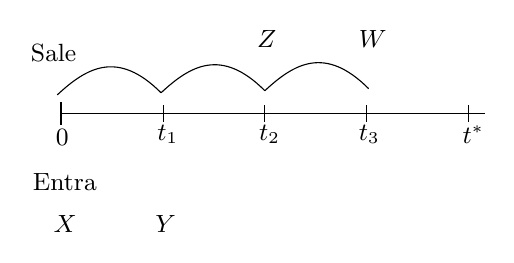
\begin{tikzpicture}[x=0.75pt,y=0.75pt,yscale=-1,xscale=1]
%uncomment if require: \path (0,300); %set diagram left start at 0, and has height of 300

%Straight Lines [id:da05634101052883045] 
\draw    (250,150.5) -- (454,150.5) (299,146.5) -- (299,154.5)(348,146.5) -- (348,154.5)(397,146.5) -- (397,154.5)(446,146.5) -- (446,154.5) ;
\draw [shift={(250,150.5)}, rotate = 180] [color={rgb, 255:red, 0; green, 0; blue, 0 }  ][line width=0.75]    (0,5.59) -- (0,-5.59)   ;
%Curve Lines [id:da25661570389460353] 
\draw    (298,140.5) .. controls (312,127.5) and (327,118.5) .. (348,139.5) ;
%Curve Lines [id:da13645212905032889] 
\draw    (348,139.5) .. controls (362,126.5) and (377,117.5) .. (398,138.5) ;
%Curve Lines [id:da3191533264218531] 
\draw    (248,141.5) .. controls (262,128.5) and (277,119.5) .. (298,140.5) ;

% Text Node
\draw (246,156.9) node [anchor=north west][inner sep=0.75pt]  [font=\small]  {$0$};
% Text Node
\draw (442,154.9) node [anchor=north west][inner sep=0.75pt]  [font=\small]  {$t^{*}$};
% Text Node
\draw (295,154.9) node [anchor=north west][inner sep=0.75pt]  [font=\small]  {$t_{1}$};
% Text Node
\draw (392,154.9) node [anchor=north west][inner sep=0.75pt]  [font=\small]  {$t_{3}$};
% Text Node
\draw (344,154.9) node [anchor=north west][inner sep=0.75pt]  [font=\small]  {$t_{2}$};
% Text Node
\draw (235,178) node [anchor=north west][inner sep=0.75pt]  [font=\small] [align=left] {Entra};
% Text Node
\draw (234,116) node [anchor=north west][inner sep=0.75pt]  [font=\small] [align=left] {Sale};
% Text Node
\draw (245,198.4) node [anchor=north west][inner sep=0.75pt]  [font=\small]  {$X$};
% Text Node
\draw (294,198.4) node [anchor=north west][inner sep=0.75pt]  [font=\small]  {$Y$};
% Text Node
\draw (343,109.4) node [anchor=north west][inner sep=0.75pt]  [font=\small]  {$Z$};
% Text Node
\draw (392,109.4) node [anchor=north west][inner sep=0.75pt]  [font=\small]  {$W$};
\end{tikzpicture}
\end{center}
¿Cuánto es el valor acumulado de todo el flujo al tiempo $t^{*}$
\begin{align*}
&\left[\left[ \left[Xa(t_1) + Y \right]a(t_2-t_1) -z\right] a(t_3-t_2) \right]a(t^{*}-t_3) \\
&=Xa(t_1)a(t_2-t_1)a(t_3-t_2)a(t^{*}-t_3)+Ya(t_2-t_1)a(t_3-t_2)a(t^{*}-t_3)\\
&-Za(t_3-t_2)a(t^{*}-t_3)- Wa(t^{*}-t_3)\\
&= \uline{X \cdot a(t^{*}) + Ya(t^{*} - t_1) -Za(t^{*}-t_2) -Wa(t^{*}-t_3)} 
\end{align*}
\item Si la fuerza de interés es constante ¿$a(t)$?

Ya vimos en general $a(t) = \exp\left\lbrace \integral{0}{t}{\delta_s}{s}\right\rbrace \mathrel{\stackon[1pt]{$=$}{$\scriptstyle\delta_t = \delta$}} \exp \left\lbrace \integral{0}{t}{\delta}{s} \right\rbrace = e^{\delta t}$

\uline{Ejemplo} (¡La tasa manda!)

Si se tiene una tasa de interés \uline{semestral} convertible \uline{mensualmente} del $9\%$, $i^{(6)}= 9\%$

El tiempo lo estamos midiendo en semestres
\begin{enumerate}
\item[1)] $a(\text{10 años}) = a(\text{20 semestres}) = \left(1 +\frac{i^{(6)}}{6} \right)^{6(20)} = \uline{\left(1+ \frac{0.09}{6} \right)^{120} }$
\item[2)] $a(\text{5 meses}) = a(\frac{5}{6} \, \text{semestre}) = \uline{\left(1+\frac{i^{(6)}}{6} \right)^{6(5/6)} }$
\item[3)]$a(\text{18 meses}) = a(\text{3 semestres}) = \left( 1+ \frac{i^{(6)}}{6}\right)^{6(3)} = \uline{\left(1 + \frac{0.09}{6} \right)^{18} } $
\end{enumerate}
\uline{Ejemplo 2} (lo mismo pero anual)
\begin{enumerate}
\item[1)] $a(\text{10 años}) = \left( 1+ \frac{i^{(12)}}{12}\right)^{12\cdot 10} = \uline{\left(1 + \frac{0.09}{12}\right)^{120} } $
\item[2)]$a(\text{5 meses}) = a\left(\frac{5}{12} \, \text{años} \right) = \uline{\left(1 + \frac{0.09}{12} \right)^5 }$
\item[3)]$a(\text{18 meses}) = a\left(\text{1.5 años} \right) = \uline{\left(1 + \frac{0.09}{12} \right)^{18} }$
\end{enumerate}
\uline{Ejemplo 3}

Tasa \uline{semestral} convertible trimestralmente del $9\%, \, i^{(2)} = 9\%$ (2 trimestres en el semestre)
\begin{enumerate}
\item[1)] $a(\text{10 años}) = a(\text{20 semestres}) = \uline{\left(1 + \frac{0.09}{2} \right)^{2\cdot 20} }$
\item[2)] $a(\text{5 meses}) = a\left(\frac{5}{6}\, \text{semestre} \right) = \uline{\left(1 + \frac{0.09}{2} \right)^{2(5/6)} }$
\item[3)] $a(\text{18 meses}) = a(\text{3 semestres}) = \uline{\left(1 + \frac{0.09}{2} \right)^{2\cdot 3} }$
\end{enumerate}
\end{enumerate}

\color{blue}\boxed{Tarea}
\color{black}
\begin{enumerate}
\item[\circled{25}] \uline{2 opciones}

La función de interés me dice si ganó o no.
\begin{center}
\tikzset{every picture/.style={line width=0.75pt}} %set default line width to 0.75pt        

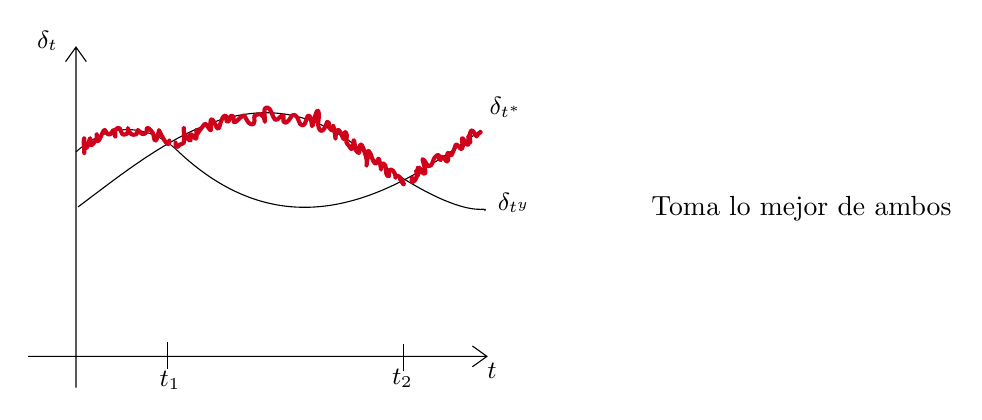
\begin{tikzpicture}[x=0.75pt,y=0.75pt,yscale=-1,xscale=1]
%uncomment if require: \path (0,300); %set diagram left start at 0, and has height of 300

%Shape: Axis 2D [id:dp11665138159327681] 
\draw  (126,199.5) -- (347,199.5)(149,50.5) -- (149,214.5) (340,194.5) -- (347,199.5) -- (340,204.5) (144,57.5) -- (149,50.5) -- (154,57.5)  ;
%Curve Lines [id:da5325745389600345] 
\draw [color={rgb, 255:red, 0; green, 0; blue, 0 }  ,draw opacity=0.92 ]   (149,101) .. controls (172,80.5) and (192,94.5) .. (198,100.5) ;
%Curve Lines [id:da9879251383651717] 
\draw    (198,100.5) .. controls (252,151.5) and (304,120.5) .. (344,90.5) ;
%Curve Lines [id:da9302740406614931] 
\draw    (150,127.5) .. controls (190,97.5) and (236,58.5) .. (287,100.5) ;
%Curve Lines [id:da49137827260961675] 
\draw    (287,100.5) .. controls (339,138.5) and (348,125.5) .. (346,129.5) ;
%Straight Lines [id:da7023570131346519] 
\draw    (193,192.5) -- (193,205.5) ;
%Straight Lines [id:da9175148700865603] 
\draw    (307,193.5) -- (307,206.5) ;
%Shape: Free Drawing [id:dp7785802603854275] 
\draw  [color={rgb, 255:red, 208; green, 2; blue, 27 }  ,draw opacity=1 ][line width=1.5] [line join = round][line cap = round] (153,94.5) .. controls (153,96.83) and (153,101.5) .. (153,101.5) .. controls (153,101.5) and (153,96.83) .. (153,94.5) .. controls (153,93.17) and (152.4,97.31) .. (153,98.5) .. controls (155.01,102.53) and (156,88.44) .. (156,97.5) .. controls (156,98.91) and (158.55,95.84) .. (159,94.5) .. controls (159.21,93.87) and (159,91.83) .. (159,92.5) .. controls (159,101.63) and (162.13,88.76) .. (163,90.5) .. controls (165.61,95.72) and (166.71,89.92) .. (167,90.5) .. controls (167.47,91.44) and (168,94.55) .. (168,93.5) .. controls (168,91.84) and (167.29,90.35) .. (169,89.5) .. controls (171.25,88.38) and (169.67,93.61) .. (173,92.5) .. controls (174.93,91.86) and (173.35,90.8) .. (174,89.5) .. controls (174.08,89.34) and (174.28,93.74) .. (178,92.5) .. controls (178.71,92.26) and (178.47,89.97) .. (179,90.5) .. controls (180.28,91.78) and (180.93,93.57) .. (183,91.5) .. controls (183.25,91.25) and (182.17,87.67) .. (185,90.5) .. controls (187.05,92.55) and (186.07,93.63) .. (187,95.5) .. controls (187.76,97.03) and (189,90.5) .. (189,90.5) .. controls (189,90.5) and (194,101.44) .. (194,95.5) ;
%Shape: Free Drawing [id:dp5030174702140806] 
\draw  [color={rgb, 255:red, 208; green, 2; blue, 27 }  ,draw opacity=1 ][line width=1.5] [line join = round][line cap = round] (197,96.5) .. controls (197,99.8) and (197.94,98.56) .. (199,97.5) .. controls (199.53,96.97) and (201,97.25) .. (201,96.5) .. controls (201,94.17) and (201,91.83) .. (201,89.5) .. controls (201,88.83) and (200.7,90.9) .. (201,91.5) .. controls (201.75,92.99) and (202.42,94.97) .. (204,95.5) .. controls (204.95,95.82) and (203.11,92.95) .. (204,92.5) .. controls (205.07,91.96) and (206.71,95.67) .. (207,94.5) .. controls (207.32,93.21) and (207,91.83) .. (207,90.5) .. controls (207,89.17) and (206.67,94.17) .. (208,91.5) .. controls (208.75,90.01) and (210.25,88.99) .. (211,87.5) .. controls (211.48,86.53) and (213.8,91.49) .. (214,90.5) .. controls (214.33,88.87) and (213.38,87.05) .. (214,85.5) .. controls (214.62,83.95) and (216.08,88.11) .. (217,89.5) .. controls (218.33,91.5) and (218.6,83.5) .. (221,83.5) .. controls (222.05,83.5) and (220.95,86.5) .. (222,86.5) .. controls (223.2,86.5) and (222.8,83.5) .. (224,83.5) .. controls (226.25,83.5) and (223.63,87.68) .. (226,86.5) .. controls (226.73,86.14) and (229.34,82.84) .. (230,83.5) .. controls (231.18,84.68) and (231.45,86.88) .. (233,87.5) .. controls (236.25,88.8) and (234.45,83.78) .. (235,83.5) .. controls (240.02,80.99) and (239.98,86.64) .. (240,86.5) .. controls (240.39,84.18) and (238.64,79.5) .. (241,79.5) .. controls (243.1,79.5) and (243.62,84.58) .. (245,85.5) .. controls (246.24,86.33) and (248.33,82.17) .. (249,83.5) .. controls (249.45,84.39) and (248.45,85.67) .. (249,86.5) .. controls (250.41,88.61) and (252.89,83.55) .. (253,83.5) .. controls (255.95,82.03) and (256.15,86.65) .. (257,87.5) .. controls (259.77,90.27) and (259.92,83.5) .. (261,83.5) .. controls (262.8,83.5) and (262.43,90.2) .. (263,88.5) .. controls (263.55,86.86) and (265.29,77.51) .. (266,82.5) .. controls (266.33,84.81) and (265.08,87.36) .. (266,89.5) .. controls (267.84,93.79) and (270,86.5) .. (270,86.5) .. controls (271.83,86.5) and (270.35,89.68) .. (272,90.5) .. controls (273.8,91.4) and (273,88.5) .. (273,88.5) .. controls (273,88.5) and (274,92.47) .. (274,94.5) .. controls (274,95.87) and (274.03,91.47) .. (275,90.5) .. controls (276.18,89.32) and (278,96.17) .. (278,94.5) .. controls (278,93.45) and (278.25,90.75) .. (279,91.5) .. controls (280.43,92.93) and (278.19,96.59) .. (280,97.5) .. controls (280.84,97.92) and (281.33,100.17) .. (282,99.5) .. controls (282.97,98.53) and (282.49,94.22) .. (283,95.5) .. controls (283.47,96.68) and (282.97,100.48) .. (285,101.5) .. controls (286.23,102.11) and (285.03,98.47) .. (286,97.5) .. controls (287.1,96.4) and (288.96,104.34) .. (289,104.5) .. controls (289.24,105.47) and (289,108.5) .. (289,107.5) .. controls (289,105.8) and (289.46,104.11) .. (290,102.5) .. controls (290.21,101.87) and (289.53,100.03) .. (290,100.5) .. controls (291.58,102.08) and (291.42,104.92) .. (293,106.5) .. controls (294.39,107.89) and (294.44,102.81) .. (295,104.5) .. controls (295.54,106.11) and (296,109.5) .. (296,109.5) .. controls (296,109.5) and (295.95,104.42) .. (298,107.5) .. controls (298.5,108.25) and (298.05,111.55) .. (299,112.5) .. controls (300.88,114.38) and (298.54,108.27) .. (301,109.5) .. controls (302.42,110.21) and (303,112.26) .. (303,113.5) .. controls (303,113.83) and (302.7,112.65) .. (303,112.5) .. controls (304.75,111.63) and (306.31,115.12) .. (307,116.5) .. controls (307.54,117.57) and (305,114.7) .. (305,113.5) ;
%Shape: Free Drawing [id:dp8120141539004881] 
\draw  [color={rgb, 255:red, 208; green, 2; blue, 27 }  ,draw opacity=1 ][line width=1.5] [line join = round][line cap = round] (311,113.5) .. controls (311,114.17) and (310.33,115.5) .. (311,115.5) .. controls (311.94,115.5) and (312.65,114.38) .. (313,113.5) .. controls (313.37,112.57) and (313,111.5) .. (313,110.5) .. controls (313,107.83) and (312.67,115.5) .. (314,111.5) .. controls (314.32,110.55) and (313,108.5) .. (314,108.5) .. controls (315.41,108.5) and (315.66,111.95) .. (317,111.5) .. controls (318.27,111.08) and (315.67,104.5) .. (316,104.5) .. controls (317.51,104.5) and (318.01,109.49) .. (320,107.5) .. controls (321,106.5) and (321,104.5) .. (322,103.5) .. controls (324.83,100.67) and (323.75,104.25) .. (324,104.5) .. controls (325.57,106.07) and (324.14,102.26) .. (326,103.5) .. controls (326.78,104.02) and (327.33,106.17) .. (328,105.5) .. controls (328.94,104.56) and (327.68,102.79) .. (328,101.5) .. controls (328.18,100.78) and (329.67,103.17) .. (330,102.5) .. controls (330.8,100.89) and (331.43,99.2) .. (332,97.5) .. controls (332.38,96.36) and (334.33,100.5) .. (335,99.5) .. controls (335.92,98.11) and (334.67,96.13) .. (335,94.5) .. controls (335.28,93.11) and (337.37,98.76) .. (338,97.5) .. controls (338.6,96.31) and (338,94.83) .. (338,93.5) .. controls (338,92.45) and (339,97.55) .. (339,96.5) .. controls (339,94.83) and (338.38,93.05) .. (339,91.5) .. controls (340.16,88.59) and (341.52,93.98) .. (342,93.5) .. controls (342.67,92.83) and (343.06,91.5) .. (344,91.5) ;

% Text Node
\draw (188,205.4) node [anchor=north west][inner sep=0.75pt]  [font=\small]  {$t_{1}$};
% Text Node
\draw (300,204.4) node [anchor=north west][inner sep=0.75pt]  [font=\small]  {$t_{2}$};
% Text Node
\draw (346,201.4) node [anchor=north west][inner sep=0.75pt]  [font=\small]  {$t$};
% Text Node
\draw (129,41.4) node [anchor=north west][inner sep=0.75pt]  [font=\small]  {$\delta _{t}$};
% Text Node
\draw (351,119.4) node [anchor=north west][inner sep=0.75pt]  [font=\small]  {$\delta _{t^{y}}$};
% Text Node
\draw (347,73.4) node [anchor=north west][inner sep=0.75pt]  [font=\small]  {$\delta _{t^{*}}$};
% Text Node
\draw (425,121) node [anchor=north west][inner sep=0.75pt]   [align=left] {Toma lo mejor de ambos};


\end{tikzpicture}
\end{center}

\item[\circled{19}]
\begin{center}
\tikzset{every picture/.style={line width=0.75pt}} %set default line width to 0.75pt        
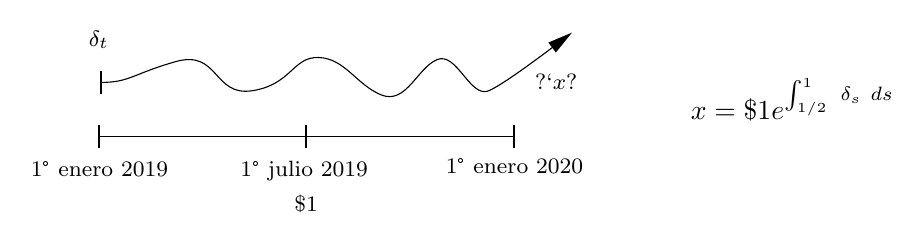
\begin{tikzpicture}[x=0.75pt,y=0.75pt,yscale=-1,xscale=1]
%uncomment if require: \path (0,300); %set diagram left start at 0, and has height of 300

%Straight Lines [id:da029038272191872494] 
\draw    (150,150.5) -- (350,150.5) ;
\draw [shift={(350,150.5)}, rotate = 180] [color={rgb, 255:red, 0; green, 0; blue, 0 }  ][line width=0.75]    (0,5.59) -- (0,-5.59)   ;
\draw [shift={(250,150.5)}, rotate = 180] [color={rgb, 255:red, 0; green, 0; blue, 0 }  ][line width=0.75]    (0,5.59) -- (0,-5.59)   ;
\draw [shift={(150,150.5)}, rotate = 180] [color={rgb, 255:red, 0; green, 0; blue, 0 }  ][line width=0.75]    (0,5.59) -- (0,-5.59)   ;
%Curve Lines [id:da10923811130555783] 
\draw    (151,124.5) .. controls (165,124.5) and (166,120.5) .. (187,114.5) .. controls (208,108.5) and (205,131.5) .. (224,128.5) .. controls (243,125.5) and (243.43,112.02) .. (256,112.5) .. controls (268.57,112.98) and (274,125.5) .. (286,130.5) .. controls (298,135.5) and (303.47,117.41) .. (313,113.5) .. controls (322.53,109.59) and (329,132.5) .. (338,128.5) .. controls (346.1,124.9) and (369.86,106.72) .. (376.48,101.66) ;
\draw [shift={(378,100.5)}, rotate = 503.13] [fill={rgb, 255:red, 0; green, 0; blue, 0 }  ][line width=0.08]  [draw opacity=0] (12,-3) -- (0,0) -- (12,3) -- cycle    ;
\draw [shift={(151,124.5)}, rotate = 180] [color={rgb, 255:red, 0; green, 0; blue, 0 }  ][line width=0.75]    (0,5.59) -- (0,-5.59)   ;

% Text Node
\draw (116,161) node [anchor=north west][inner sep=0.75pt]  [font=\footnotesize] [align=left] {1° enero 2019};
% Text Node
\draw (217,161) node [anchor=north west][inner sep=0.75pt]  [font=\footnotesize] [align=left] {1° julio 2019};
% Text Node
\draw (316,160) node [anchor=north west][inner sep=0.75pt]  [font=\footnotesize] [align=left] {1° enero 2020};
% Text Node
\draw (243,177.4) node [anchor=north west][inner sep=0.75pt]  [font=\footnotesize]  {$\text{\textdollar}1$};
% Text Node
\draw (359,119.4) node [anchor=north west][inner sep=0.75pt]  [font=\footnotesize]  {$\text{¿}x\text{?}$};
% Text Node
\draw (144,98.4) node [anchor=north west][inner sep=0.75pt]  [font=\footnotesize]  {$\delta _{t}$};
% Text Node
\draw (434,121.4) node [anchor=north west][inner sep=0.75pt]    {$x=\text{\textdollar}1e^{\int _{1/2}^{1} \ \delta _{s} \ ds}$};
\end{tikzpicture}
\end{center}
\newpage
\color{blue}\boxed{Ejercicios}
\color{black}
\item[\circled{3}] El concepto de tasa equivalente solo existe para $\delta_t$ constante.

$1 + 0.005(12) = (1+i)^1$

$1 + 0.005(1/12) = (1+i)^{1/12}$

\end{enumerate}

\chapter*{Anualidades}
Considere la siguiente transacción:

Se deposita $\$1$ cada periodo durante $n$ periodos, i.e, hay $n$ depósitos de $\$1$.
 \begin{enumerate}[label=\protect\circled{\arabic*}]
 \item Supongamos interés compuesto, ¿cuánto dinero acumulado se tiene justo después del último depósito?
\begin{center}
\tikzset{every picture/.style={line width=0.75pt}} %set default line width to 0.75pt        
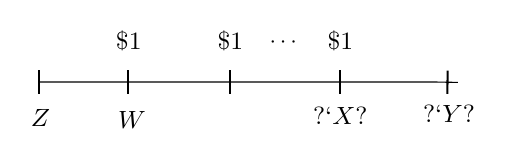
\begin{tikzpicture}[x=0.75pt,y=0.75pt,yscale=-1,xscale=1]
%uncomment if require: \path (0,300); %set diagram left start at 0, and has height of 300

%Straight Lines [id:da8832358581674458] 
\draw    (251,151.33) -- (337,151.33) -- (349,151.33) -- (443,151.33) -- (453,151.5) ;
\draw [shift={(294,151.33)}, rotate = 540] [color={rgb, 255:red, 0; green, 0; blue, 0 }  ][line width=0.75]    (0,5.59) -- (0,-5.59)   ;
\draw [shift={(343,151.33)}, rotate = 540] [color={rgb, 255:red, 0; green, 0; blue, 0 }  ][line width=0.75]    (0,5.59) -- (0,-5.59)   ;
\draw [shift={(396,151.33)}, rotate = 540] [color={rgb, 255:red, 0; green, 0; blue, 0 }  ][line width=0.75]    (0,5.59) -- (0,-5.59)   ;
\draw [shift={(448,151.41)}, rotate = 180.99] [color={rgb, 255:red, 0; green, 0; blue, 0 }  ][line width=0.75]    (0,5.59) -- (0,-5.59)   ;
\draw [shift={(251,151.33)}, rotate = 540] [color={rgb, 255:red, 0; green, 0; blue, 0 }  ][line width=0.75]    (0,5.59) -- (0,-5.59)   ;

% Text Node
\draw (361,128.6) node [anchor=north west][inner sep=0.75pt]  [font=\footnotesize] [align=left] {$\displaystyle \cdots $};
% Text Node
\draw (246,163.4) node [anchor=north west][inner sep=0.75pt]  [font=\small]  {$Z$};
% Text Node
\draw (288,164.4) node [anchor=north west][inner sep=0.75pt]  [font=\small]  {$W$};
% Text Node
\draw (435,161.4) node [anchor=north west][inner sep=0.75pt]  [font=\small]  {$\text{¿} Y\text{?}$};
% Text Node
\draw (287,125.4) node [anchor=north west][inner sep=0.75pt]  [font=\small]  {$\text{\textdollar}1$};
% Text Node
\draw (336,125.4) node [anchor=north west][inner sep=0.75pt]  [font=\small]  {$\text{\textdollar}1$};
% Text Node
\draw (389,125.4) node [anchor=north west][inner sep=0.75pt]  [font=\small]  {$\text{\textdollar}1$};
% Text Node
\draw (382,162.4) node [anchor=north west][inner sep=0.75pt]  [font=\small]  {$\text{¿} X\text{?}$};
\end{tikzpicture}
\end{center}
\begin{itemize}
\item[$\cdot$] Justo después del $2\text{°}$ depósito, ¿cuánto dinero acumulado hay?

$1(1+i)^1+\underbrace{1}_{\scriptstyle \text{peso adicional}}$
\item[$\cdot$] Justo después del $3\text{°}$ depósito, ¿cuánto dinero tenemos?

$\underbrace{\left[1(1+i)^1 + 1 \right]}_{\scriptstyle \text{Ya lo teníamos}}(1+i) + \underbrace{1}_{\scriptstyle \text{peso adicional}} = (1+i)^2 +(1+i) +1 $
\item[$\cdot$] Justo después del $4\text{°}$ depósito, ¿cuánto?

$\left[(1+i)^2 + (1+i) +1 \right](1+i) +1 = (1+i)^3 +(1+i)^2 + (1+i) +1 $
\end{itemize}

Inductivamente, justo después del $n\text{-ésimo}$ depósito, ¿cuánto dinero tenemos?
$$=\underbrace{(1+i)^{n-1}+(1+i)^{n-2}+\ldots+(1+i) +1 = x}_{\scriptstyle n\, \text{sumandos}}$$

\item ¿Cuánto dinero hay un periodo después del último depósito?
\begin{align*}
&X(1+i) = Y\\
Y &= (1+i)\left[(1+i)^{n-1} + (1+i)^{n-2}+ \ldots + (1+i) +1 \right] \\
&= \underbrace{(1+i)^n + (1+i)^{n-1} + \ldots + (1+i)}_{\scriptstyle n\, \text{sumandos}}
\end{align*}
\item Si en vez de esa maroma de hacer $n$ depósitos y simplemente hacer \uline{un único depósito} en la misma fecha del $1\text{°}$ pago y obtener el mismo valor acumulado.

¿De cuánto tendría que ser este depósito?
\begin{align*}
&W\,\text{debe satisfacer:} \: W(1+i)^n = Y\\
&\text{ó bien} \, W(1+i)^{n-1} = X \: \Longrightarrow \: W=Y(1+i)^n\\
& W = \left[(1+i)^n + (1+i)^{n-1}+\ldots + (1+i) \right] (1+i)^{-n}\\
&= \underbrace{1+ (1+i)^{-1} + \ldots + (1+i)^{-(n-1)}}_{\scriptstyle n\, \text{sumandos}} 
\end{align*}
\item Si en vez de esa maroma de hacer $n$ depósitos y simplemente hacer \uline{un único depósito} un periodo antes de la fecha del $1\text{°}$ pago. 

¿De cuánto debe ser dicho depósito?
\begin{align*}
&Z\,\text{debe satisfacer:}\: Z(1+i)^n=X \: \text{ó bien} \: Z(1+i)^{n+1} = Y\\
& \Longrightarrow \: Z= X(1+i)^{-n} = \left[(1+i)^{n-1} + (1+i)^{n-2} + \ldots + (1+i) + 1 \right](1+i)^{-n}\\
&\hspace{1.5cm} = (1+i)^{-1} +(1+i)^{-2} +\ldots +(1+i)^{-(n-1)} + (1+i)^{-n} = (*) 
\end{align*}
\end{enumerate}
\uline{Notación}

$(*)=\underbrace{V+V^2+\ldots + V^{n-1}+V^n}_{\scriptstyle n\, \text{sumandos}} $

\uline{En resumen}
\begin{enumerate}[label=\protect\circled{\arabic*}]
\item $X=(1+i)^{n-1}+(1+i)^{n-2}+\ldots+(1+i) +1 \: \color{red}: \sx{\angln i}$
\color{black} \item $Y = (1+i)^n + (1+i)^{n-1}+\ldots+(1+i) \: \: \color{red}: \sx**{\angln i}$
\color{black} \item $W = 1 + V + V^2 + \ldots + V^{n-1} \: \color{red}: \ax**{\angln i}$
\color{black} \item $Z = V+V^2+\ldots +V^n \: \color{red}: \ax{\angln i}$

\color{red}$i \: \longrightarrow  \: \text{tasa efectiva de interés por periodo}\\
n \: \longrightarrow \: \text{número de pagos}$

\color{black}$\sx{\angln i}, \, \ax**{\angln i}, \, \sx**{\angln i}, \, \ax{\angln i}, \, n\in \NN$

\end{enumerate}
\color{blue}\boxed{Ejercicios}
\color{black}
\begin{enumerate}
\item[\circled{2}] Se sabe que una inversión de $\$500$ se incrementará a $\$4000$ al final de $30$ años. Encontrar la suma de valores presentes de 3 pagos de $\$10,000$ cada uno, los cuales se harán al final de $20$, $40$ y $60$ años, con la tasa del ejercicio anterior.
\begin{center}
\tikzset{every picture/.style={line width=0.75pt}} %set default line width to 0.75pt        
\begin{tikzpicture}[x=0.75pt,y=0.75pt,yscale=-1,xscale=1]
%uncomment if require: \path (0,300); %set diagram left start at 0, and has height of 300

%Straight Lines [id:da9028571471300229] 
\draw    (101,150.5) -- (250,150.5) (200,146.5) -- (200,154.5) ;
\draw [shift={(252,150.5)}, rotate = 180] [color={rgb, 255:red, 0; green, 0; blue, 0 }  ][line width=0.75]    (10.93,-3.29) .. controls (6.95,-1.4) and (3.31,-0.3) .. (0,0) .. controls (3.31,0.3) and (6.95,1.4) .. (10.93,3.29)   ;
\draw [shift={(101,150.5)}, rotate = 180] [color={rgb, 255:red, 0; green, 0; blue, 0 }  ][line width=0.75]    (0,5.59) -- (0,-5.59)   ;
%Straight Lines [id:da8872512598854625] 
\draw    (300,150.5) -- (450,150.5) (350,146.5) -- (350,154.5)(400,146.5) -- (400,154.5) ;
\draw [shift={(450,150.5)}, rotate = 180] [color={rgb, 255:red, 0; green, 0; blue, 0 }  ][line width=0.75]    (0,5.59) -- (0,-5.59)   ;
\draw [shift={(300,150.5)}, rotate = 180] [color={rgb, 255:red, 0; green, 0; blue, 0 }  ][line width=0.75]    (0,5.59) -- (0,-5.59)   ;

% Text Node
\draw (122,141) node [anchor=north west][inner sep=0.75pt]   [align=left] {$ $};
% Text Node
\draw (97,92) node [anchor=north west][inner sep=0.75pt]   [align=left] {I};
% Text Node
\draw (296,91) node [anchor=north west][inner sep=0.75pt]   [align=left] {II};
% Text Node
\draw (103,153.9) node [anchor=north west][inner sep=0.75pt]  [font=\footnotesize]  {$0$};
% Text Node
\draw (193,159.4) node [anchor=north west][inner sep=0.75pt]  [font=\footnotesize]  {$30\ \text{Años}$};
% Text Node
\draw (186,129.9) node [anchor=north west][inner sep=0.75pt]  [font=\footnotesize]  {$4000$};
% Text Node
\draw (296,159.9) node [anchor=north west][inner sep=0.75pt]  [font=\footnotesize]  {$0$};
% Text Node
\draw (343,159.9) node [anchor=north west][inner sep=0.75pt]  [font=\footnotesize]  {$20$};
% Text Node
\draw (392,160.9) node [anchor=north west][inner sep=0.75pt]  [font=\footnotesize]  {$40$};
% Text Node
\draw (443,159.9) node [anchor=north west][inner sep=0.75pt]  [font=\footnotesize]  {$60$};
% Text Node
\draw (295,175.9) node [anchor=north west][inner sep=0.75pt]  [font=\footnotesize]  {$X$};
% Text Node
\draw (333,129.9) node [anchor=north west][inner sep=0.75pt]  [font=\footnotesize]  {$10000$};
% Text Node
\draw (382,129.9) node [anchor=north west][inner sep=0.75pt]  [font=\footnotesize]  {$10000$};
% Text Node
\draw (433,129.9) node [anchor=north west][inner sep=0.75pt]  [font=\footnotesize]  {$10000$};
\end{tikzpicture}
\end{center}
\begin{align*}
\Longrightarrow \: &500(1+i)^{30} = 4000 \: \Longrightarrow \: (1+i)^{30} = 8 \: \Longrightarrow \: i = \ldots \\
x &= 10,000 V^20 + 10,000 V^40 +10,000 V^60 \\
&= 10,000\left[(1+i)^{-20} + (1+i)^{-40} + (1+i)^{-60} \right]\\
&= \uline{10,000\left[8^{-2/3} + 8^{-4/3} + 8^{-2} \right]}\\
&\hfill \\
&\text{donde} \: 1+i = 8^{1/30} 
\end{align*}
\item[\circled{3}] \begin{enumerate}
\item Encuentre $d_s$ si la tasa de interés simple es $10\%$
\item Encuentre $d_s$ si la tasa de descuento simple es $10\%$
\end{enumerate}
\item[a)] \begin{align*}
a(t)& = 1+0.1t\\
ds& = \frac{a(5)-a(4)}{a(5)}\\
& = \frac{1+0.1(5) -1 -0.1(4)}{1+0.1(4)}\\
& = \uline{\frac{0.1}{1.5}}
\end{align*}
\item[b)] Análogo pero con tasa de descuento.
\end{enumerate}

\begin{lemma}
Para $x\in \RR, \, k, \, n \in \NN_+, \, k<n$. Sea $S= x^k + x^{k+1} + \ldots + x^n$, entonces
$$\color{red}\boxed{\color{black}S = \frac{x^k-x^{n+1}}{1-x}}$$
\color{blue} $\cdot$ Las fórmulas de las anualidades se deducen de este lema.
\end{lemma}
\color{black} \begin{proof}
\begin{align*}
& S = x^k + x^{k+1} + \ldots + x^n \\
& xS = \hspace{0.5cm} x^{k+1} + \ldots + x^n + x^{n+1} \\
& \Longrightarrow S-xS = x^k -x^{n+1} \\
& \Longrightarrow S = \frac{x^k-x^{n+1}}{1-x} 
\end{align*}
\end{proof}
\begin{center}
\tikzset{every picture/.style={line width=0.75pt}} %set default line width to 0.75pt        
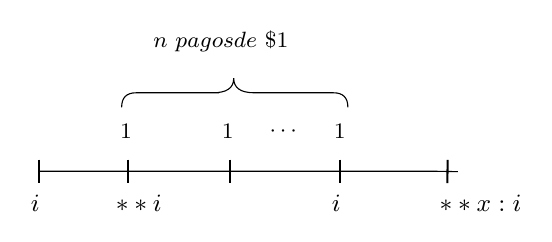
\begin{tikzpicture}[x=0.75pt,y=0.75pt,yscale=-1,xscale=1]
%uncomment if require: \path (0,300); %set diagram left start at 0, and has height of 300

%Straight Lines [id:da7121791548097758] 
\draw    (251,151.33) -- (337,151.33) -- (349,151.33) -- (443,151.33) -- (453,151.5) ;
\draw [shift={(294,151.33)}, rotate = 540] [color={rgb, 255:red, 0; green, 0; blue, 0 }  ][line width=0.75]    (0,5.59) -- (0,-5.59)   ;
\draw [shift={(343,151.33)}, rotate = 540] [color={rgb, 255:red, 0; green, 0; blue, 0 }  ][line width=0.75]    (0,5.59) -- (0,-5.59)   ;
\draw [shift={(396,151.33)}, rotate = 540] [color={rgb, 255:red, 0; green, 0; blue, 0 }  ][line width=0.75]    (0,5.59) -- (0,-5.59)   ;
\draw [shift={(448,151.41)}, rotate = 180.99] [color={rgb, 255:red, 0; green, 0; blue, 0 }  ][line width=0.75]    (0,5.59) -- (0,-5.59)   ;
\draw [shift={(251,151.33)}, rotate = 540] [color={rgb, 255:red, 0; green, 0; blue, 0 }  ][line width=0.75]    (0,5.59) -- (0,-5.59)   ;
%Shape: Brace [id:dp9632853672475934] 
\draw   (400,120.5) .. controls (400,115.83) and (397.67,113.5) .. (393,113.5) -- (355,113.5) .. controls (348.33,113.5) and (345,111.17) .. (345,106.5) .. controls (345,111.17) and (341.67,113.5) .. (335,113.5)(338,113.5) -- (298,113.5) .. controls (293.33,113.5) and (291,115.83) .. (291,120.5) ;

% Text Node
\draw (361,128.6) node [anchor=north west][inner sep=0.75pt]  [font=\footnotesize] [align=left] {$\displaystyle \cdots $};
% Text Node
\draw (246,161.4) node [anchor=north west][inner sep=0.75pt]  [font=\small]  {$\ax{\angln i}$};
% Text Node
\draw (287,161.4) node [anchor=north west][inner sep=0.75pt]  [font=\small]  {$\ax**{\angln i}$};
% Text Node
\draw (443,161.4) node [anchor=north west][inner sep=0.75pt]  [font=\small]  {$\sx**{x:\angln i} $};
% Text Node
\draw (289,127.4) node [anchor=north west][inner sep=0.75pt]  [font=\footnotesize]  {$1$};
% Text Node
\draw (338,127.4) node [anchor=north west][inner sep=0.75pt]  [font=\footnotesize]  {$1$};
% Text Node
\draw (392,127.4) node [anchor=north west][inner sep=0.75pt]  [font=\footnotesize]  {$1$};
% Text Node
\draw (391,161.4) node [anchor=north west][inner sep=0.75pt]  [font=\small]  {$\sx{\angln i} $};
% Text Node
\draw (305,82.4) node [anchor=north west][inner sep=0.75pt]  [font=\footnotesize]  {$n\ \text{pagos de} \ \text{\textdollar}1$};


\end{tikzpicture}
\end{center}
\begin{proposition}
\hfill
\begin{enumerate}
\item[1)] Si $i \neq 0$, entonces
$\color{red}\boxed{\color{black}\ax{\angln i} = \frac{1-V^n}{i}} \color{black} = \frac{1-(1+i)^{-n}}{i}$
\item[2)] Si $i \neq 0$, entonces $\color{red}\boxed{\color{black}\ax**{\angln i} = \frac{1-V^n}{d}} \color{black} = \frac{1-(1+i)^{-n}}{d}$, donde $d \sim i$
\item[3)] Si $i \neq 0$, entonces $\color{red}\boxed{\color{black}\sx{\angln i} = \frac{(1+i)^n -1}{i}} \color{black}$
\item[4)] Si $i \neq 0$, entonces $\color{red}\boxed{\color{black}\sx**{\angln i} = \frac{(1+i)^n -1}{d}} \color{black}$, con $d\sim i$
\item[5)] Si $i = 0$, entonces $\ax{\angln} = \ax**{\angln} = \sx{\angln} = \sx**{\angln}$
\end{enumerate}
\end{proposition} 
\begin{proof}
\begin{align*}
1) \quad \ax{\angln i} &= V + V^2 + \ldots + V^n = V^1 + V^2 + \ldots + V^n \mathrel{\stackon[1pt]{$=$}{$\scriptstyle \text{lema}$}} \frac{V^1 - V^{n+1}}{1-V}\\
&= \frac{V\left(1-V^n\right)}{V\left[(1+i) -1\right]} = \frac{1-V^n}{i}\\
&\hfill \\
2) \quad \ax**{\angln i} &= 1 + V + V^2 + \ldots + V^{n-1} = V^0 + V + V^2 + \ldots + V^{n-1} \mathrel{\stackon[1pt]{$=$}{$\scriptstyle \text{lema}$}} \frac{V^0 - V^{n-1+1}}{1-V}\\
&= \frac{1-V^n}{1-V} \: \ldots \: (\Smiley) \quad \text{pero} \, d\sim i, \, (1-d)^{-1} = 1+i \Longrightarrow 1-d = \frac{1}{1+i}\\
\Longrightarrow \: &d = 1 - \frac{1}{1+i} = 1 - V \: \ldots \: (\Sadey)\\
\text{Sust.}\, &(\Smiley) \, \text{en} \, (\Sadey)\\
\ax**{\angln i} &= \frac{1-V^n}{d}\\
&\hfill \\
3) \quad \sx{\angln i} &= 1+(1+i) + \ldots + (1+i)^{n-1} = (1+i)^0 + (1+i)^1 + \ldots + (1+i)^{n-1}\\
& \mathrel{\stackon[1pt]{$=$}{$\scriptstyle \text{lema}$}} \frac{(1+i)^0 - (1+i)^{n-1+1}}{1-(1+i)} = \frac{1-(1+i)^n}{-i} = \frac{(1+i)^n - 1}{i}\\
4) \quad \sx**{\angln i} &= (1+i) + (1+i)^2 + \ldots +(1+i)^n \mathrel{\stackon[1pt]{$=$}{$\scriptstyle \text{lema}$}} \frac{(1+i)^1 - (1+i)^{n+1}}{1-(1+i)} \\
& = \frac{-(1+i)\left[-1 + (1+i)^n \right] }{-i} \: \Longrightarrow \: \sx**{\angln i} = \frac{(1+i)\left[(1+i)^n - 1\right] }{i} \: \ldots \: (\heartsuit)\\
\text{Pero como} &\: i\sim d, \, (1+i)=(1-d)^{-1} \: \Longrightarrow \: d=1- \frac{1}{1+i} = \frac{1+i-1}{1+i} = \frac{i}{1+i}\\
\Longrightarrow\: \frac{1}{d} &= \frac{1+i}{i} \: \ldots \: (\rotatebox[origin=c]{180}{\ensuremath\heartsuit})\\
\text{Sust.}\, (\rotatebox[origin=c]{180}{\ensuremath\heartsuit}) \, &\text{en} \, (\heartsuit)\\
\sx**{\angln i} &= \frac{1}{d}\left[(1+i)^n - 1 \right] = \frac{(1+i)^n-1}{d}\\ 
&\hfill\\
5) \quad \sx{\angln i} &= 1 + (1+i) \ldots + (1+i)^{n-1} = 1+(1+0) + \ldots + (1+0)^{n-1}\\
&= 1+1\ldots+1=n\\
\ax{\angln i} &= V+V^2+\ldots+V^n = (1+i)^{-1} + (1+i)^{-2} +\ldots + (1+i)^{-n}\\
&\mathrel{\stackon[1pt]{$=$}{$\scriptstyle i=1$}} 1^{-1} + 1^{-2} + \ldots + 1^{-n} = 1 + \ldots + 1=n
\end{align*}
\end{proof}
\text{Ahora}

\begin{align*}
r(Ga)_{\angln i} &= \underbrace{1V + (1+r)V^2 + (1+r)^2V^3 + \ldots + (1+r)^{n-2}V^{n-1} + (1+r)^{n-1}V^n}_{\scriptstyle n \, \text{sumandos}} \\
&= V\left[ 1+(1+r)V + [(1+r)V]^2 + \ldots + [(1+r)V]^{n-2} + [(1+r)V]^{n-1}\right]\\
& \mathrel{\stackon[1.5pt]{$=$}{$\scriptstyle \text{lema}$}} V\left[\frac{[(1+r)V]^0 - [(1+r)V]^{n-1+1}}{1-(1+r)V} \right] \: \longleftarrow \: x = (1+r)V\\
&= V\left[\frac{1-(1+r)^nV^n}{1-(1+r)V} \right] = \frac{1-(1+r)^nV^n}{V^{-1}[1-(1+r)V]} = \frac{1-(1+r)^nV^n}{V^{-1}-(1+r)} \\
& = \frac{1-(1+r)^n V^n}{(1+i)-(1+r)} = \color{red}\boxed{\color{black}\frac{1-\left(\frac{1+r}{1+i} \right)^n }{1-r}, \: i \neq r}\\
&\hfill\\
r(G\sx**{})_{\angln i} &\mathrel{\stackon[1.5pt]{$=$}{$\scriptstyle \text{Def}$}} (1+r)^{n-1}(1+i) + (1+r)^{n-2}(1+i)^2 + \ldots + (1+r)^2(1+i)^{n-2} \\
&\quad + (1+r)(1+i)^{n-1} + 1(1+i)^n \\
&= (1+r)^n \left[\frac{1+i}{1+r} + \left(\frac{1+i}{1+r} \right)^2 + \ldots + \left( \frac{1+i}{1+r} \right)^n  \right] \\
&\mathrel{\stackon[1.5pt]{$=$}{$\scriptstyle \text{lema}$}} (1+r)^n \left[\frac{\left(\frac{1+i}{1+r} \right)^1 - \left( \frac{1+i}{1+r} \right)^{n+1} }{1 - \left(\frac{1+i}{1+r} \right) } \right] \: \longleftarrow \: x = \frac{1+i}{1+r}\\
& = \frac{(1+r)^n\left( \frac{1+i}{1+r}\right)\left[1 - \left(\frac{1+i}{1+r} \right)^n  \right]  }{\frac{1+r-1-i}{1+r}} = \frac{(1+i)(1+r)^{n-1}\left[1 - \frac{(1+i)^n}{(1+r)^n}  \right] }{\frac{r-i}{1+r}}\\
&= \frac{(1+i)(1+r)^n\left[1 - \frac{(1+i)^n}{(1+r)^n} \right] }{r-i} = \frac{(1+i)\left[(1+r)^n - (1+i)^n \right] }{r-i}\\
& = \color{red}\boxed{\color{black}\frac{(1+i)^n - (1+r)^n}{\frac{i-r}{1+i}}}
\end{align*}
\begin{center}
\tikzset{every picture/.style={line width=0.75pt}} %set default line width to 0.75pt        
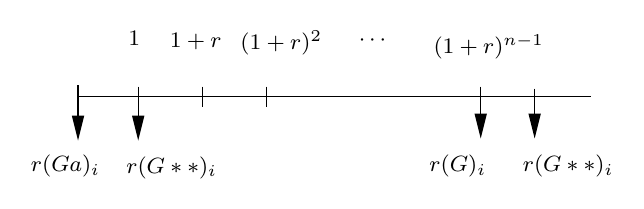
\begin{tikzpicture}[x=0.75pt,y=0.75pt,yscale=-1,xscale=1]
%uncomment if require: \path (0,300); %set diagram left start at 0, and has height of 300

%Straight Lines [id:da43824497554422015] 
\draw    (181,150.5) -- (428,150.5) ;
\draw [shift={(181,150.5)}, rotate = 180] [color={rgb, 255:red, 0; green, 0; blue, 0 }  ][line width=0.75]    (0,5.59) -- (0,-5.59)   ;
%Straight Lines [id:da07100029549462694] 
\draw    (210,145.5) -- (210,155.5) ;
%Straight Lines [id:da2510178303998858] 
\draw    (241,145.5) -- (241,155.5) ;
%Straight Lines [id:da34030264746251615] 
\draw    (272,145.5) -- (272,155.5) ;
%Straight Lines [id:da013278159215051044] 
\draw    (375,145.5) -- (375,155.5) ;
%Straight Lines [id:da8466290982042055] 
\draw    (401,146.5) -- (401,156.5) ;
%Straight Lines [id:da043487341685954695] 
\draw    (210,155.5) -- (210,169.5) ;
\draw [shift={(210,171.5)}, rotate = 270] [fill={rgb, 255:red, 0; green, 0; blue, 0 }  ][line width=0.08]  [draw opacity=0] (12,-3) -- (0,0) -- (12,3) -- cycle    ;
%Straight Lines [id:da4984835167102657] 
\draw    (375,152.5) -- (375,168.5) ;
\draw [shift={(375,170.5)}, rotate = 270] [fill={rgb, 255:red, 0; green, 0; blue, 0 }  ][line width=0.08]  [draw opacity=0] (12,-3) -- (0,0) -- (12,3) -- cycle    ;
%Straight Lines [id:da5388030033804363] 
\draw    (401,153.5) -- (401,168.5) ;
\draw [shift={(401,170.5)}, rotate = 270] [fill={rgb, 255:red, 0; green, 0; blue, 0 }  ][line width=0.08]  [draw opacity=0] (12,-3) -- (0,0) -- (12,3) -- cycle    ;
%Straight Lines [id:da3856299368597913] 
\draw    (181,150.5) -- (181,169.5) ;
\draw [shift={(181,171.5)}, rotate = 270] [fill={rgb, 255:red, 0; green, 0; blue, 0 }  ][line width=0.08]  [draw opacity=0] (12,-3) -- (0,0) -- (12,3) -- cycle    ;

% Text Node
\draw (204,117.4) node [anchor=north west][inner sep=0.75pt]  [font=\footnotesize]  {$1$};
% Text Node
\draw (224,118.4) node [anchor=north west][inner sep=0.75pt]  [font=\footnotesize]  {$1+r$};
% Text Node
\draw (258,117.4) node [anchor=north west][inner sep=0.75pt]  [font=\footnotesize]  {$( 1+r)^{2}$};
% Text Node
\draw (315,119.4) node [anchor=north west][inner sep=0.75pt]  [font=\footnotesize]  {$\cdots $};
% Text Node
\draw (351,119.4) node [anchor=north west][inner sep=0.75pt]  [font=\footnotesize]  {$( 1+r)^{n-1}$};
% Text Node
\draw (157,177.4) node [anchor=north west][inner sep=0.75pt]  [font=\footnotesize]  {$r(Ga)_{\angln i}$};
% Text Node
\draw (203,177.9) node [anchor=north west][inner sep=0.75pt]  [font=\footnotesize]  {$r(G\ax**{})_{\angln i}$};
% Text Node
\draw (349,177.4) node [anchor=north west][inner sep=0.75pt]  [font=\footnotesize]  {$r(G\sx{})_{\angln i}$};
% Text Node
\draw (394,177.4) node [anchor=north west][inner sep=0.75pt]  [font=\footnotesize]  {$r(G\sx**{})_{\angln i}$};
\end{tikzpicture}
\end{center}

\begin{proposition}
\hfill
\begin{enumerate}
\item[1)] Si $i\neq r, \: r(Ga)_{\angln i} = \frac{1- \left(\frac{1+r}{1+i} \right)^n }{i-r}$
\item[2)] Si $i\neq r, \: r(G\ax**{})_{\angln i} = \frac{1- \left(\frac{1+r}{1+i} \right)^n}{\frac{i-r}{1+i}}$
\item[3)] Si $i\neq r, \: r(G\sx{})_{\angln i} = \frac{(1+i)^n - (1+r)^n}{i-r}$
\item[4)] Si $i\neq r, \: r(G\sx**{})_{\angln i} = \frac{(1+i)^n - (1+r)^n}{\frac{i-r}{1+i}}$
\item[5)] Si $i= r,  \: r(G\ax**{})_{\angln i} = r(Ga)_{\angln i} = r(G\sx{})_{\angln i} = r(G\sx**{})_{\angln i} = n  $
\end{enumerate}
\end{proposition}
\begin{align*}
r(G\ax**{})_{\angln i}  &\mathrel{\stackon[1.5pt]{$=$}{$\scriptstyle \text{Def}$}} 1 + (1+r)V + (1+r)^2V^2 + \ldots + (1+r)^{n-1}V^{n-1}\\
&= 1 + \frac{1+r}{1+i} + \left(\frac{1+r}{1+i} \right)^2 + \ldots + \left( \frac{1+r}{1+i} \right)^{n-1}\\
& \mathrel{\stackon[1.5pt]{$=$}{$\scriptstyle i = r$}} 1 + \frac{1+i}{1+i} + \left(\frac{1+i}{1+i} \right)^2 + \ldots + \left(\frac{1+i}{1+i} \right)^n = 1+ \ldots + 1 = n  
\end{align*}
\color{blue}\boxed{Ejercicios}
\color{black}
\begin{enumerate}
\item Supóngase que el incremento del dinero para los siguientes $5$ años está dado a una tasa de descuento del $5\%$.
\begin{enumerate}
\item ¿Cuál es la cantidad de dinero que se debería invertir hoy para tener $\$23,000$ en $3$ años?
\item Se desea invertir una cantidad $2$ años, para tener $\$23,000$ en $5$ años ¿Cuál es esa cantidad de dinero?
\end{enumerate}
\begin{center}
\tikzset{every picture/.style={line width=0.75pt}} %set default line width to 0.75pt        
\begin{tikzpicture}[x=0.75pt,y=0.75pt,yscale=-1,xscale=1]
%uncomment if require: \path (0,300); %set diagram left start at 0, and has height of 300

%Straight Lines [id:da6774419389486246] 
\draw    (401,151.5) -- (550,151.5) ;
\draw [shift={(550,151.5)}, rotate = 180] [color={rgb, 255:red, 0; green, 0; blue, 0 }  ][line width=0.75]    (0,5.59) -- (0,-5.59)   ;
\draw [shift={(401,151.5)}, rotate = 180] [color={rgb, 255:red, 0; green, 0; blue, 0 }  ][line width=0.75]    (0,5.59) -- (0,-5.59)   ;
%Curve Lines [id:da9666398552325044] 
\draw    (401,151.5) .. controls (440.6,121.8) and (503.72,121.5) .. (548.64,150.61) ;
\draw [shift={(550,151.5)}, rotate = 213.69] [fill={rgb, 255:red, 0; green, 0; blue, 0 }  ][line width=0.08]  [draw opacity=0] (12,-3) -- (0,0) -- (12,3) -- cycle    ;

% Text Node
\draw (395,154.4) node [anchor=north west][inner sep=0.75pt]  [font=\small]  {$x$};
% Text Node
\draw (532,157.4) node [anchor=north west][inner sep=0.75pt]  [font=\small]  {$3\ \text{años}$};
% Text Node
\draw (535,122.4) node [anchor=north west][inner sep=0.75pt]  [font=\small]  {$23,000$};
% Text Node
\draw (120,93.4) node [anchor=north west][inner sep=0.75pt]    {$\text{a)} \ \ \ a( t) \ =\ ( 1-0.05)^{t} \ $};
% Text Node
\draw (124,130.4) node [anchor=north west][inner sep=0.75pt]    {$x\cdot a\left( 3\ \text{años}\right) \ =\ 23,000\ $};
% Text Node
\draw (101,161.4) node [anchor=north west][inner sep=0.75pt]    {$\Longrightarrow x=\frac{23,000}{a( 3)} \ =\ \underline{\frac{23,000}{( 1-0.05)^{-3}}}$};


\end{tikzpicture}
\end{center}
\begin{center}
\tikzset{every picture/.style={line width=0.75pt}} %set default line width to 0.75pt        
\begin{tikzpicture}[x=0.75pt,y=0.75pt,yscale=-1,xscale=1]
%uncomment if require: \path (0,300); %set diagram left start at 0, and has height of 300

%Straight Lines [id:da1052145717361439] 
\draw    (400,151.5) -- (549,151.5) ;
\draw [shift={(549,151.5)}, rotate = 180] [color={rgb, 255:red, 0; green, 0; blue, 0 }  ][line width=0.75]    (0,5.59) -- (0,-5.59)   ;
\draw [shift={(400,151.5)}, rotate = 180] [color={rgb, 255:red, 0; green, 0; blue, 0 }  ][line width=0.75]    (0,5.59) -- (0,-5.59)   ;
%Straight Lines [id:da6184109190263691] 
\draw    (438,146.5) -- (438,156.5) ;

% Text Node
\draw (396,157.4) node [anchor=north west][inner sep=0.75pt]  [font=\small]  {$x$};
% Text Node
\draw (531,157.4) node [anchor=north west][inner sep=0.75pt]  [font=\small]  {$5\ \text{años}$};
% Text Node
\draw (534,122.4) node [anchor=north west][inner sep=0.75pt]  [font=\small]  {$23,000$};
% Text Node
\draw (433,159.4) node [anchor=north west][inner sep=0.75pt]  [font=\small]  {$1$};
% Text Node
\draw (112,94.4) node [anchor=north west][inner sep=0.75pt]    {$\text{b)} \ \ \ y\ \text{satisface} \ $};
% Text Node
\draw (115,131.4) node [anchor=north west][inner sep=0.75pt]    {$y\cdot a( 5-2) \ =\ 23,000\ $};
% Text Node
\draw (92,162.4) node [anchor=north west][inner sep=0.75pt]    {$\Longrightarrow y=\frac{23,000}{a( 3)} \ =\ \underline{\frac{23,000}{( 1-0.05)^{-3}}}$};
% Text Node
\draw (450.5,145.9) node [anchor=north west][inner sep=0.75pt]    {$\dotsc $};
% Text Node
\draw (468.5,145.9) node [anchor=north west][inner sep=0.75pt]    {$\dotsc $};
% Text Node
\draw (485.5,145.9) node [anchor=north west][inner sep=0.75pt]    {$\dotsc $};


\end{tikzpicture}
\end{center}
\item Regina garantiza un pago de $5,000$ en $4$ años. Ella necesita $\$4,500$ ahora con el fin de pagar su colegiatura. El mejor préstamos para Regina es una tasa de descuento del $4.9\%$ para pagar la cantidad de $\$5,501.62$ en exactamente $4$ años. Ella puede cubrir $\$5,000$ de su pago garantizado y añadir $\$501.62$ extras al final de los $4$ años. Alternativamente, Regina podría vender su pago garantizado y usar la ganancia para cubrir el total de su colegiatura. ¿En cuánto debería estar dispuesta a vender su pago?
\begin{center}
\tikzset{every picture/.style={line width=0.75pt}} %set default line width to 0.75pt        
\begin{tikzpicture}[x=0.75pt,y=0.75pt,yscale=-1,xscale=1]
%uncomment if require: \path (0,300); %set diagram left start at 0, and has height of 300

%Straight Lines [id:da762690760878286] 
\draw    (444,150.5) -- (593,150.5) ;
\draw [shift={(593,150.5)}, rotate = 180] [color={rgb, 255:red, 0; green, 0; blue, 0 }  ][line width=0.75]    (0,5.59) -- (0,-5.59)   ;
\draw [shift={(444,150.5)}, rotate = 180] [color={rgb, 255:red, 0; green, 0; blue, 0 }  ][line width=0.75]    (0,5.59) -- (0,-5.59)   ;

% Text Node
\draw (425,158.4) node [anchor=north west][inner sep=0.75pt]  [font=\small]  {$4,000$};
% Text Node
\draw (578,121.4) node [anchor=north west][inner sep=0.75pt]  [font=\small]  {$5,000$};
% Text Node
\draw (462,124) node [anchor=north west][inner sep=0.75pt]  [font=\footnotesize] [align=left] {Regina garantizado };
% Text Node
\draw (44,124.4) node [anchor=north west][inner sep=0.75pt]    {$ \begin{array}{l}
\text{Nótese que} \ \ 4500( 1-d)^{-4} =4500( 1-0.049)^{-4}\\
\ \ \ \ \ \ \ \ \ \ \ \ \ \ \ \ \ \ \ \ \ \ \ \ \ \ \ \ \ \ \ \ \ \ \ \ \ \ \ \ \ \ =\ 5,501.61
\end{array}$};


\end{tikzpicture}
\end{center}
\begin{align*}
&\text{\uline{Primero:}}\\
& \text{¿Cuál es la i que satisface:}\, 4500(1+i)^4 = 5000 \, \text{?}\\
&\Longrightarrow\: i = \left(\frac{10}{9} \right)^{1/4} = 0.02669 \: \Longrightarrow \: i = 2.2669\%\\
&\text{¿Cuál es la tasa de descuento equivalente} \, d^* \, \text{?}\\
&(1-d^*) = 1+i\\
&d^* = 1-V = 1 - \frac{1}{1+i} = \frac{i}{1+i} = \frac{0.02669}{1.02669} = 0.025\\
&\Longrightarrow\: \uline{d>d^*} 
\end{align*}
\end{enumerate}





\chapter*{Referencias}

\end{document}